\documentclass[11pt,a4paper]{report}

\usepackage[T1]{fontenc}
\usepackage[utf8]{inputenc}
\usepackage{mathptmx}
\usepackage[scaled=0.9]{helvet}
\usepackage{courier}
\DeclareFontFamily{T1}{pcrs}{\hyphenchar\font=-1}
\DeclareFontShape{T1}{pcrs}{m}{n}{<->s*[0.84]pcrr8t}{}
\DeclareFontShape{T1}{pcrs}{m}{sl}{<->s*[0.84]pcrro8t}{}
\DeclareFontShape{T1}{pcrs}{m}{it}{<->ssub*pcrs/m/sl}{}
\DeclareFontShape{T1}{pcrs}{b}{n}{<->s*[0.84]pcrb8t}{}
\DeclareFontShape{T1}{pcrs}{bx}{n}{<->ssub*pcrs/b/n}{}
\renewcommand{\ttdefault}{pcrs}
\usepackage[margin=2.4cm,top=2.4cm,bottom=2.4cm]{geometry}
\usepackage{microtype}
\usepackage{amsmath,amssymb,mathtools}
\usepackage{graphicx}
\usepackage{booktabs}
\usepackage{array}
\usepackage{tabularx}
\usepackage{longtable}
\usepackage{xcolor}
\usepackage{enumitem}
\usepackage{fancyhdr}
\usepackage{titlesec}
\usepackage{tikz}
\usetikzlibrary{arrows.meta,positioning,shapes.geometric,calc,fit,decorations.pathreplacing}
\usepackage[most]{tcolorbox}
\usepackage{listings}
\usepackage[hidelinks,pdfusetitle]{hyperref}
\usepackage{caption}

\setlist{itemsep=2pt,topsep=4pt}
\setlength{\parindent}{0pt}
\setlength{\parskip}{6pt}
\captionsetup{font=small,labelfont=bf}

% ---------- colours
\definecolor{accent}{HTML}{1F5FA8}
\definecolor{plainbg}{HTML}{EEF5FC}
\definecolor{soundbg}{HTML}{EAF6EC}
\definecolor{soundfg}{HTML}{2E7D32}
\definecolor{warnbg}{HTML}{FFF4E0}
\definecolor{warnfg}{HTML}{B26A00}
\definecolor{codebg}{HTML}{F7F7F7}
\definecolor{codecomment}{HTML}{4F7F4F}

% ---------- boxes
\newtcolorbox{plain}[1][In plain words]{enhanced,breakable,colback=plainbg,colframe=accent,
  boxrule=0.5pt,left=6pt,right=6pt,top=4pt,bottom=4pt,fonttitle=\bfseries\small,title={#1}}
\newtcolorbox{sound}[1][Interview soundbite]{enhanced,breakable,colback=soundbg,colframe=soundfg,
  boxrule=0.5pt,left=6pt,right=6pt,top=4pt,bottom=4pt,fonttitle=\bfseries\small,title={#1}}
\newtcolorbox{warn}[1][Careful]{enhanced,breakable,colback=warnbg,colframe=warnfg,
  boxrule=0.5pt,left=6pt,right=6pt,top=4pt,bottom=4pt,fonttitle=\bfseries\small,title={#1}}

% ---------- code listings
\lstdefinestyle{cpp}{language=C++,basicstyle=\ttfamily\footnotesize,columns=fullflexible,keepspaces=true,
  breaklines=true,breakatwhitespace=false,commentstyle=\color{codecomment}\itshape,keywordstyle=\color{accent}\bfseries,
  backgroundcolor=\color{codebg},frame=single,rulecolor=\color{black!20},framesep=4pt,xleftmargin=4pt,xrightmargin=4pt,
  showstringspaces=false,aboveskip=6pt,belowskip=6pt}
\lstdefinestyle{shell}{language=bash,basicstyle=\ttfamily\footnotesize,columns=fullflexible,keepspaces=true,breaklines=true,
  backgroundcolor=\color{codebg},frame=single,rulecolor=\color{black!20},framesep=4pt,xleftmargin=4pt,xrightmargin=4pt,
  commentstyle=\color{codecomment}\itshape,showstringspaces=false,aboveskip=6pt,belowskip=6pt,
  morekeywords={sbatch,salloc,squeue,scancel,module,make,rsync,ssh,scp,ws_allocate,ws_find,ws_list,ws_extend,srun}}
\lstset{style=cpp}
\DeclareRobustCommand{\_}{\textunderscore\allowbreak{}}
\emergencystretch=2em
\newcommand{\inputrows}[1]{\input{#1}\\ \bottomrule}
\newcommand{\code}[1]{\texttt{#1}}
\newcommand{\file}[1]{\texttt{#1}}

% ---------- headings / header
\titleformat{\chapter}[display]{\normalfont\huge\bfseries\color{accent}}{\chaptertitlename\ \thechapter}{8pt}{\Huge}
\titlespacing*{\chapter}{0pt}{-10pt}{18pt}
\titleformat{\section}{\normalfont\Large\bfseries\color{accent}}{\thesection}{0.7em}{}
\titleformat{\subsection}{\normalfont\large\bfseries}{\thesubsection}{0.7em}{}
\pagestyle{fancy}\fancyhf{}
\fancyhead[L]{\small\nouppercase{\leftmark}}\fancyhead[R]{\small SIMD Image Processing Library}
\fancyfoot[C]{\small\thepage}
\renewcommand{\headrulewidth}{0.3pt}

\newcommand{\sbxCpu}{Intel(R) Xeon(R) Processor @ 2.10GHz}
\newcommand{\sbxCompiler}{g++ (Ubuntu 13.3.0-6ubuntu2~24.04.1) 13.3.0}
\newcommand{\sbxDate}{2026-10-07}
\newcommand{\betweenScalarMed}{28}
\newcommand{\betweenScalarMax}{48}
\newcommand{\betweenAutovecMed}{11}
\newcommand{\betweenAutovecMax}{33}
\newcommand{\betweenAvxMed}{2}
\newcommand{\betweenAvxMax}{13}
\newcommand{\repSpreadOne}{15}
\newcommand{\repSpreadTwo}{17}
\newcommand{\msGrayScalar}{4.52}
\newcommand{\spGrayAutovec}{1.0}
\newcommand{\spGrayAvx}{3.9}
\newcommand{\spGrayAvxTwo}{7.4}
\newcommand{\spGrayScalarTwo}{1.9}
\newcommand{\scGrayAvx}{1.89}
\newcommand{\msSobelScalar}{8.10}
\newcommand{\spSobelAutovec}{3.6}
\newcommand{\spSobelAvx}{7.8}
\newcommand{\spSobelAvxTwo}{15.0}
\newcommand{\spSobelScalarTwo}{2.0}
\newcommand{\scSobelAvx}{1.94}
\newcommand{\msConvThreeScalar}{37.39}
\newcommand{\spConvThreeAutovec}{1.0}
\newcommand{\spConvThreeAvx}{18.0}
\newcommand{\spConvThreeAvxTwo}{34.8}
\newcommand{\spConvThreeScalarTwo}{2.0}
\newcommand{\scConvThreeAvx}{1.93}
\newcommand{\msConvFiveScalar}{77.72}
\newcommand{\spConvFiveAutovec}{0.9}
\newcommand{\spConvFiveAvx}{16.6}
\newcommand{\spConvFiveAvxTwo}{33.2}
\newcommand{\spConvFiveScalarTwo}{2.0}
\newcommand{\scConvFiveAvx}{2.00}
\newcommand{\msConvNineScalar}{202.30}
\newcommand{\spConvNineAutovec}{0.8}
\newcommand{\spConvNineAvx}{14.6}
\newcommand{\spConvNineAvxTwo}{28.8}
\newcommand{\spConvNineScalarTwo}{2.0}
\newcommand{\scConvNineAvx}{1.97}
\newcommand{\msConvElevenScalar}{304.32}
\newcommand{\spConvElevenAutovec}{0.8}
\newcommand{\spConvElevenAvx}{15.3}
\newcommand{\spConvElevenAvxTwo}{29.2}
\newcommand{\spConvElevenScalarTwo}{2.0}
\newcommand{\scConvElevenAvx}{1.91}
\newcommand{\gfAvxThree}{37}
\newcommand{\gfAvxNine}{52}
\newcommand{\gfAvxMax}{58}
\newcommand{\gfScalarMax}{3.3}
\newcommand{\gfRowAccNine}{8.0}
\newcommand{\gfRowAccMax}{13}
\newcommand{\ratioAccFourNine}{1.14}
\newcommand{\ratioAccFourMax}{1.30}
\newcommand{\ratioPerTapNine}{1.44}
\newcommand{\ratioRowAccToAvx}{6.5}
\newcommand{\ratioRowAccToNatural}{3.2}
\newcommand{\nominalPeakGf}{67}
\newcommand{\fracOfNominalPeak}{86}
\newcommand{\mpixGrayAvxSmall}{3680}
\newcommand{\mpixGrayAvxHuge}{1772}
\newcommand{\mpixSobelAvxSmall}{3516}
\newcommand{\mpixSobelAvxHuge}{3626}
\newcommand{\mpixGrayScalarMin}{838}
\newcommand{\mpixGrayScalarMax}{935}
\newcommand{\copyOneBig}{25}
\newcommand{\copyTwoBig}{50}
\newcommand{\copyOneSmall}{65}
\newcommand{\gbGrayAvxFourK}{14.6}
\newcommand{\gbSobelAvxFourK}{8.4}
\newcommand{\pctGrayOfCopy}{58}
\newcommand{\pctSobelOfCopy}{34}
\newcommand{\pctGrayOfCopyTwo}{55}
\newcommand{\scaleGrayAvxFourK}{1.91}
\newcommand{\scaleConvAvxFourK}{1.95}
\newcommand{\scaleSobelAvxFourK}{1.94}
\newcommand{\strideWorstSlow}{16}
\newcommand{\strideBestFast}{-11}
\newcommand{\ocvGray}{1.5}
\newcommand{\ocvSobel}{8.3}
\newcommand{\ocvConvThree}{2.0}
\newcommand{\ocvConvNine}{2.5}
\newcommand{\mutKilled}{12}
\newcommand{\mutTotal}{12}
\newcommand{\gccVec}{2}
\newcommand{\testChecks}{4\,269\,710}
\newcommand{\testFailures}{0}
\newcommand{\testGroups}{24}
\newcommand{\errBoundRatio}{0.092}
\newcommand{\crossComparisons}{786}
\newcommand{\crossMismatches}{0}
\newcommand{\crossApproxPct}{0.00070}
\newcommand{\crossApproxWorst}{1}


\begin{document}

% ============================================================ title page
\begin{titlepage}
\centering
\vspace*{2.2cm}
{\Huge\bfseries\color{accent} SIMD Image Processing Library\par}
\vspace{0.3cm}
{\LARGE CPU optimization: scalar, OpenMP, AVX2\par}
\vspace{0.4cm}
{\LARGE The complete guide\par}
\vspace{0.8cm}
{\large what it is, why it is fast, how the code does it,\\ how to run it on bwUniCluster, and how to talk about it\par}
\vspace{1.4cm}
\begin{tcolorbox}[colback=plainbg,colframe=accent,width=0.82\textwidth,boxrule=0.5pt]
\raggedright
\textbf{Written for:} Syed Akram Ameer Abbas\\
\textbf{Project:} ``SIMD Image Processing Library -- CPU Optimization'' (C++, AVX2, OpenMP, Python), project 1 on the resume\\
\textbf{Level of the implementation:} what a solid M.Sc.\ graduate in an embedded / computing programme would build: readable, tested, measured, and honest about its limits\\
\textbf{Target:} bwUniCluster 3.0 (KIT), GNU toolchain, Slurm\\
\textbf{Code:} the \file{simd\_imgproc/} directory delivered together with this PDF
\end{tcolorbox}
\vfill
{\small Everything printed in this guide as a number, table, figure or listing was produced by the code in the project:\\
no value was typed in by hand. Where a number is \emph{yours to measure} (the cluster benchmarks), the guide says so.\par}
\end{titlepage}

\tableofcontents

% ============================================================ chapters
\chapter{The big picture}\label{ch:overview}

\section{What you built, in three sentences}

You built a small C++ library that performs three classic image operations on 8-bit pictures: \textbf{colour to gray conversion}, \textbf{Sobel edge detection} and \textbf{2D convolution} (blur, sharpen, \dots\ with kernels of any odd size). Each operation exists in several versions that compute \emph{exactly the same thing} but use the processor differently: plain scalar code, the same code with the compiler's auto-vectorizer switched on, hand-written \textbf{AVX2} instructions that handle 8 to 32 numbers at once, and each of these split across several CPU cores with \textbf{OpenMP}. Then you measured how much faster each version is, checked that it is still correct, and looked for the reasons.

\begin{plain}
The one-sentence version for an interview: \emph{``I implemented grayscale, Sobel and 2D convolution in scalar, OpenMP and AVX2 form, proved the fast versions equal to a simple reference, and measured speedup, throughput and where each kernel is limited by compute or by memory.''}
\end{plain}

\section{The three operations and the four ways of running them}

\begin{center}
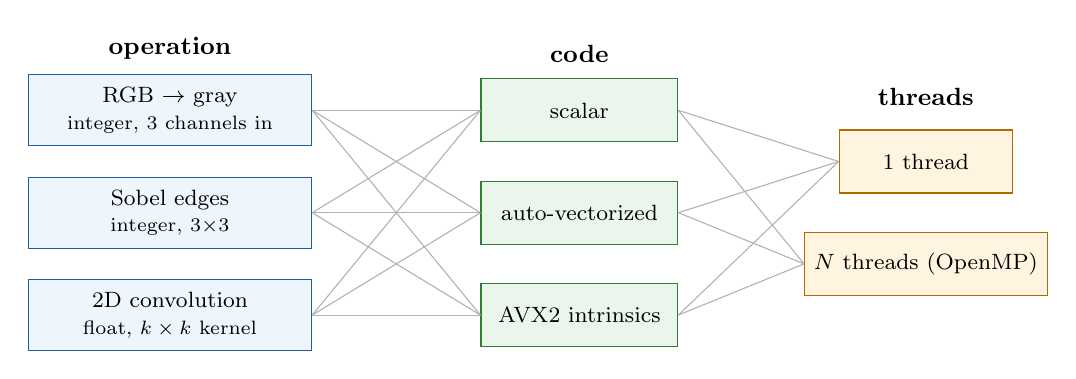
\begin{tikzpicture}[x=1cm,y=1cm,font=\footnotesize,
  op/.style={draw=accent,fill=plainbg,minimum width=3.6cm,minimum height=0.9cm,align=center},
  im/.style={draw=soundfg,fill=soundbg,minimum width=2.5cm,minimum height=0.8cm,align=center},
  th/.style={draw=warnfg,fill=warnbg,minimum width=2.2cm,minimum height=0.8cm,align=center}]
\node[op] (g) at (0,0) {RGB $\to$ gray\\\scriptsize integer, 3 channels in};
\node[op] (s) at (0,-1.3) {Sobel edges\\\scriptsize integer, 3$\times$3};
\node[op] (c) at (0,-2.6) {2D convolution\\\scriptsize float, $k\times k$ kernel};
\node[im] (i1) at (5.2,0.0) {scalar};
\node[im] (i2) at (5.2,-1.3) {auto-vectorized};
\node[im] (i3) at (5.2,-2.6) {AVX2 intrinsics};
\node[th] (t1) at (9.6,-0.65) {1 thread};
\node[th] (t2) at (9.6,-1.95) {$N$ threads (OpenMP)};
\foreach \a in {g,s,c} \foreach \b in {i1,i2,i3} \draw[gray!60] (\a.east) -- (\b.west);
\foreach \a in {i1,i2,i3} \foreach \b in {t1,t2} \draw[gray!60] (\a.east) -- (\b.west);
\node[above=2pt of g,font=\small\bfseries] {operation};
\node[above=2pt of i1,font=\small\bfseries] {code};
\node[above=2pt of t1,font=\small\bfseries,yshift=3pt] {threads};
\end{tikzpicture}
\end{center}

Every operation is available in every combination ($3\times3\times2$). The \emph{correctness contract} is: all combinations produce the same pixels. For gray and Sobel the results are identical bit for bit. For convolution the AVX2 result is identical to a reference that uses fused multiply-adds, and the scalar result differs from it by at most one grey level in a handful of rare cases that this guide explains (Chapter~\ref{ch:numerics}).

\section{What this project is and is not}

Being precise about scope makes you more credible, so here it is plainly.

\begin{itemize}
\item \textbf{It is} a complete, tested, measured CPU-optimization study: three kernels, scalar/OpenMP/AVX2 implementations, a reference-based test suite (over 4 million checks including an exhaustive test of all 16.7 million RGB colours), a benchmark harness with a memory-bandwidth yardstick, and experiments on caches, strides, kernel sizes and threads.
\item \textbf{It is not} a replacement for OpenCV, Intel IPP or NVIDIA NPP. It handles 8-bit images only, one border mode (edge replication), and square odd kernels. It does not use AVX-512, does not do tiling across multiple rows at once, and does not implement separable-kernel shortcuts. Chapter~\ref{ch:bench} compares it with OpenCV on one machine so you can speak about the gap honestly.
\item \textbf{The numbers in this PDF} were measured in the sandbox where the code was written (a virtual machine with two cores). They show \emph{what the experiments look like and how to read them}. The \textbf{bwUniCluster numbers are yours to measure}: Chapter~\ref{ch:cluster} gives the exact steps and the scripts. Never quote a sandbox number as a cluster number.
\end{itemize}

\begin{warn}[Honesty rule for the interview]
Say ``SIMD image processing library, grayscale / Sobel / convolution, scalar vs.\ OpenMP vs.\ AVX2'' exactly as the resume does. Anyone who knows SIMD will respect a precise list of what you implemented and what you deliberately left out far more than a vague claim like ``a high-performance imaging library''.
\end{warn}

\section{Where everything lives}

\begin{center}
\small
\begin{tabular}{@{}p{5.5cm}p{9.2cm}@{}}
\toprule
\textbf{File} & \textbf{What it does}\\ \midrule
\file{include/simdip/image.hpp}, \file{src/image.cpp} & \code{Image}: aligned rows, stride, PNM file I/O, synthetic test images.\\
\file{include/simdip/kernel.hpp}, \file{src/kernel.cpp} & Filter kernels (box, Gaussian, binomial, sharpen, \dots) and their validation.\\
\file{include/simdip/ops.hpp} & The public API: \code{rgbToGray}, \code{sobel}, \code{convolve}, plus the reference and ablation functions.\\
\file{src/scalar\_impl.inc} & The plain C++ code. Compiled twice: \file{scalar\_novec.cpp} (vectorizer off) and \file{scalar\_autovec.cpp} (vectorizer on).\\
\file{src/avx2.cpp} & Hand-written AVX2 kernels.\\
\file{src/dispatch.cpp} & Argument checks, CPU feature check, splitting rows over OpenMP threads.\\
\file{src/reference.cpp} & Slow, obviously-correct reference implementations used by the tests.\\
\file{apps/simdip\_cli.cpp}, \file{apps/simdip\_bench.cpp} & Command line tool; benchmark harness (CSV output).\\
\file{tests/test\_main.cpp} & 24 test groups, no framework needed.\\
\file{python/ref\_numpy.py}, \file{crosscheck.py} & Independent NumPy/SciPy model and the C++ vs.\ NumPy comparison.\\
\file{python/compare\_opencv.py} & Agreement and speed comparison with OpenCV.\\
\file{python/run\_experiments.py} & Runs experiments E1--E5 and writes the CSVs.\\
\file{slurm/*.sbatch} & Job scripts for bwUniCluster 3.0.\\ \bottomrule
\end{tabular}
\end{center}

\section{How to use this guide}

\begin{enumerate}
\item Read Chapters~\ref{ch:images}--\ref{ch:math} slowly, with the code open next to you. They explain the pictures, the three operations and the maths in plain language.
\item Chapters~\ref{ch:scalar}--\ref{ch:conv} walk through the code: scalar, OpenMP, the SIMD basics, and the three AVX2 kernels.
\item Chapters~\ref{ch:cache}--\ref{ch:testing} are the engineering: cache behaviour, numerical accuracy, testing. This is what turns ``I wrote intrinsics'' into ``I know why it is fast and why it is correct''.
\item Chapter~\ref{ch:bench} shows the measurements; Chapter~\ref{ch:cluster} is the step-by-step bwUniCluster guide. Chapters~\ref{ch:resume}--\ref{ch:drills} are the interview material.
\end{enumerate}
Each chapter ends with an \textbf{Interview soundbite} you can say aloud in thirty seconds.

\chapter{Step 0: what an image is, to a computer}\label{ch:images}

\section{Pixels are bytes}

A grayscale picture is a grid of numbers from 0 (black) to 255 (white). One number fits in one \emph{byte} (8 bits), and that byte is called a \emph{pixel}. A colour picture has three numbers per pixel: how much red, green and blue light. A $1920\times1080$ gray image is about 2\,MB; the same picture in colour is about 6\,MB.

\begin{plain}
\textbf{Why 8 bits?} It is what cameras, screens and JPEG files use, and it keeps the data small. The price is that arithmetic on pixels easily overflows: $200+100$ does not fit in a byte. Much of the care in this project is about doing arithmetic in wider types (16-bit integers or 32-bit floats) and converting back with \emph{clamping} (values above 255 become 255, below 0 become 0).
\end{plain}

\section{How the grid is laid out in memory}

Memory is a long line of bytes, so the 2D grid has to be flattened. We store it \textbf{row by row} (``row-major''), and for colour images the three channels of one pixel sit next to each other (``interleaved'': \code{R G B R G B \dots}).

\begin{center}
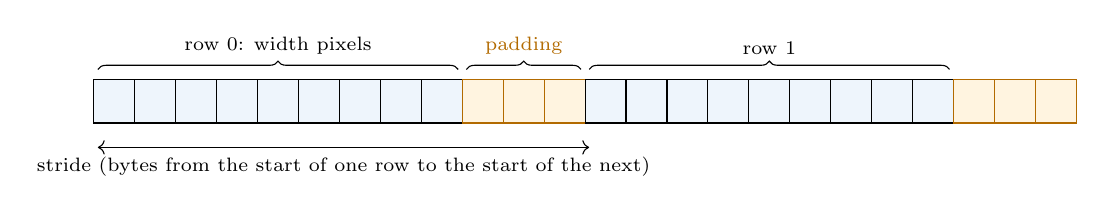
\begin{tikzpicture}[x=0.52cm,y=0.9cm,font=\scriptsize]
\foreach \i in {0,...,8} { \node[draw,fill=plainbg,minimum width=0.52cm,minimum height=0.55cm,inner sep=0] at (\i,0) {}; }
\foreach \i in {9,10,11} { \node[draw,fill=warnbg,draw=warnfg,minimum width=0.52cm,minimum height=0.55cm,inner sep=0] at (\i,0) {}; }
\foreach \i in {12,...,20} { \node[draw,fill=plainbg,minimum width=0.52cm,minimum height=0.55cm,inner sep=0] at (\i,0) {}; }
\foreach \i in {21,22,23} { \node[draw,fill=warnbg,draw=warnfg,minimum width=0.52cm,minimum height=0.55cm,inner sep=0] at (\i,0) {}; }
\draw[decorate,decoration={brace,amplitude=3pt}] (-0.4,0.45) -- node[above=2pt]{row 0: \code{width} pixels} (8.4,0.45);
\draw[decorate,decoration={brace,amplitude=3pt,raise=0pt}] (8.6,0.45) -- node[above=2pt,text=warnfg]{padding} (11.4,0.45);
\draw[decorate,decoration={brace,amplitude=3pt}] (11.6,0.45) -- node[above=2pt]{row 1} (20.4,0.45);
\draw[<->] (-0.4,-0.65) -- node[below]{\code{stride} (bytes from the start of one row to the start of the next)} (11.6,-0.65);
\end{tikzpicture}
\end{center}

The address of the pixel in column $x$ and row $y$ is
\[
\text{address}(x,y)=\text{base}+y\cdot\text{stride}+x\cdot\text{channels}.
\]
The \textbf{stride} is at least the row length, and may be larger: the extra bytes are \emph{padding}. Real image libraries do this for two reasons, and so does this one:
\begin{enumerate}
\item \textbf{Alignment}: every row starts at a multiple of 64 bytes (the size of a cache line), which makes vector loads and stores efficient.
\item \textbf{Avoiding a cache trap}: if the stride is an exact multiple of 4096 bytes (a page), rows that are read together can fight for the same few cache slots. \code{Image::defaultStride()} adds one cache line in that case (Chapter~\ref{ch:cache} measures whether it matters on your machine).
\end{enumerate}
The kernels never read or write the padding as pixels; a test fills the padding with a marker value and checks that it is unchanged afterwards (\code{outputs\_never\_touch\_the\_row\_padding}).

\section{The Image class}

\lstinputlisting{snippets/code_image_class.cpp}

Notes on what a reviewer looks for: ownership is by a \code{unique\_ptr} with a custom deleter (no leaks, no manual \code{free}); copying is deep, moving is cheap; the constructor validates sizes; memory is touched (zeroed) at construction so that page faults happen \emph{before} any timing starts; and \code{alignedAlloc} requests the \emph{exact} number of bytes, so a sanitizer (AddressSanitizer) sees where the buffer really ends and reports a vector load that reads even one byte too far.

\section{What happens at the edges?}

A $3\times3$ filter looking at a pixel in the first column needs a neighbour that does not exist. Some choice must be made; the choice is a \emph{border mode}. Ours is \textbf{replicate} (also called ``clamp to edge''): a missing pixel takes the value of the nearest real one. This is OpenCV's \code{BORDER\_REPLICATE}, and it never invents dark or bright values.

\begin{center}
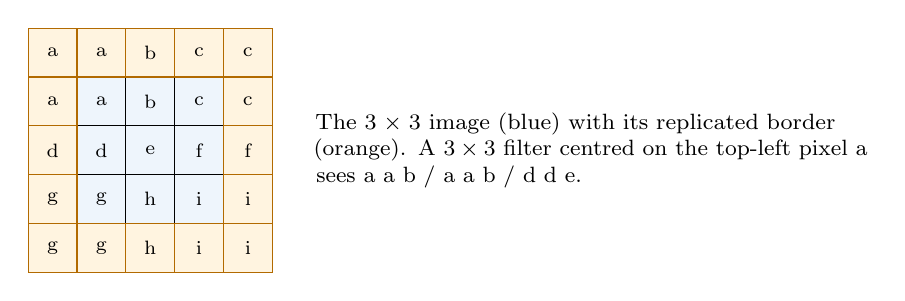
\begin{tikzpicture}[x=0.62cm,y=0.62cm,font=\scriptsize]
\foreach \x/\y/\v in {0/0/a,1/0/b,2/0/c,0/1/d,1/1/e,2/1/f,0/2/g,1/2/h,2/2/i} {
  \node[draw,fill=plainbg,minimum size=0.62cm,inner sep=0] at (\x,-\y) {\v};
}
\foreach \y in {0,1,2} { \node[draw,fill=warnbg,draw=warnfg,minimum size=0.62cm,inner sep=0] at (-1,-\y) {\ifcase\y a\or d\or g\fi};
                         \node[draw,fill=warnbg,draw=warnfg,minimum size=0.62cm,inner sep=0] at (3,-\y) {\ifcase\y c\or f\or i\fi}; }
\foreach \x in {0,1,2} { \node[draw,fill=warnbg,draw=warnfg,minimum size=0.62cm,inner sep=0] at (\x,1) {\ifcase\x a\or b\or c\fi};
                         \node[draw,fill=warnbg,draw=warnfg,minimum size=0.62cm,inner sep=0] at (\x,-3) {\ifcase\x g\or h\or i\fi}; }
\foreach \px/\py/\v in {-1/1/a,3/1/c,-1/-3/g,3/-3/i} { \node[draw,fill=warnbg,draw=warnfg,minimum size=0.62cm,inner sep=0] at (\px,\py) {\v}; }
\node[anchor=west,font=\footnotesize,text width=7cm] at (4.2,-1) {The $3\times3$ image (blue) with its replicated border (orange). A $3\times3$ filter centred on the top-left pixel \code{a} sees \code{a a b / a a b / d d e}.};
\end{tikzpicture}
\end{center}

\begin{sound}
``Images are stored row-major with a stride, 64-byte aligned rows, and edge-replicated borders. The stride is padded so rows are cache-line aligned and never an exact multiple of a page; the kernels never touch the padding, which a test verifies.''
\end{sound}

\chapter{The three operations: maths in plain language}\label{ch:math}

\section{RGB to gray}

\subsection{The idea}

Gray is a weighted average of red, green and blue. The weights are not equal because the human eye is most sensitive to green and least to blue. The standard (ITU-R BT.601) weights are
\[
Y = 0.299\,R + 0.587\,G + 0.114\,B .
\]
A pure green pixel therefore looks much brighter in gray than a pure blue one of the same intensity.

\subsection{Doing it with integers only}

Floating-point is not needed, and integer arithmetic is easier to make exact and fast. Multiply the three weights by 256 and round: $0.299\cdot256=76.5\to77$, $0.587\cdot256=150.3\to150$, $0.114\cdot256=29.2\to29$. These add up to exactly $256$, so a white pixel stays white ($255\cdot256/256=255$). Dividing by 256 is the same as shifting right by 8 bits:
\begin{equation}
Y=\Big\lfloor\frac{77R+150G+29B+128}{256}\Big\rfloor=(77R+150G+29B+128)\gg 8 .
\end{equation}
The ``$+128$'' is half of 256: it turns the floor (rounding down) into rounding to the nearest integer. The coefficients are the ones JPEG-style converters use; the quick check is
\[
R=255,G=0,B=0\;\Rightarrow\;(77\cdot255+128)\gg8=19\,763\gg8=77,\qquad
R=G=B=255\;\Rightarrow\;(65\,280+128)\gg 8=255 .
\]

\begin{plain}
\textbf{Why this matters for SIMD.} The largest possible intermediate value is $77\cdot255+150\cdot255+29\cdot255+128=65\,408$, which is smaller than $2^{16}=65\,536$. So the whole computation fits in \emph{unsigned 16-bit} numbers and a 256-bit register can hold 16 of them at once. The test \code{gray\_exhaustive\_all\_16777216\_colours} runs every one of the $256^3$ colours through every implementation: a proof by exhaustion, not a sample.
\end{plain}

\section{2D convolution}

\subsection{The idea}

A \emph{kernel} is a small grid of weights, for example $3\times3$. To filter an image, slide the kernel over every pixel; at each position multiply the weights with the pixels underneath, add up, and write the sum to the output pixel.

\begin{center}
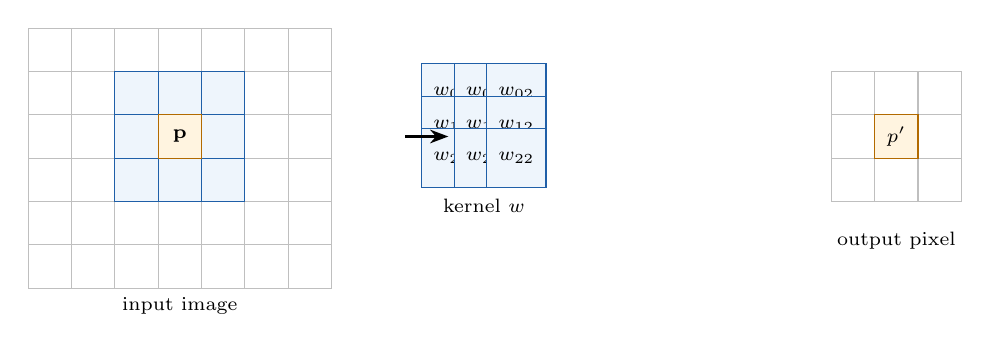
\begin{tikzpicture}[x=0.55cm,y=0.55cm,font=\scriptsize]
\foreach \x in {0,...,6}\foreach \y in {0,...,5}{ \node[draw=gray!50,minimum size=0.55cm,inner sep=0] at (\x,-\y) {}; }
\foreach \x in {2,3,4}\foreach \y in {1,2,3}{ \node[draw=accent,fill=plainbg,minimum size=0.55cm,inner sep=0] at (\x,-\y) {}; }
\node[draw=warnfg,fill=warnbg,minimum size=0.55cm,inner sep=0] at (3,-2) {\textbf{p}};
\node at (3,-5.9) {input image};
\begin{scope}[xshift=5.1cm]
\foreach \x/\y/\v in {0/0/w_{00},1/0/w_{01},2/0/w_{02},0/1/w_{10},1/1/w_{11},2/1/w_{12},0/2/w_{20},1/2/w_{21},2/2/w_{22}}{
 \node[draw=accent,fill=plainbg,minimum size=0.75cm,inner sep=0] at (\x*0.75,-\y*0.75-1) {$\v$}; }
\node at (0.75,-3.6) {kernel $w$};
\end{scope}
\draw[-{Stealth},thick] (8.2,-2.0) -- (9.2,-2.0);
\begin{scope}[xshift=10.2cm]
\foreach \x in {0,...,2}\foreach \y in {0,...,2}{ \node[draw=gray!50,minimum size=0.55cm,inner sep=0] at (\x,-\y-1) {}; }
\node[draw=warnfg,fill=warnbg,minimum size=0.55cm,inner sep=0] at (1,-2) {$p'$};
\node at (1,-4.4) {output pixel};
\end{scope}
\end{tikzpicture}
\end{center}

In formulas, for a kernel of size $k=2r+1$:
\begin{equation}
\text{out}(x,y)=\operatorname{clamp}\Big(\operatorname{round}\Big(\sum_{j=0}^{k-1}\sum_{i=0}^{k-1} w_{ji}\;\text{in}(x+i-r,\;y+j-r)\Big),\,0,\,255\Big).
\end{equation}
Each output pixel costs $k^2$ multiplications and $k^2$ additions: $3\times3$ is 9, $9\times9$ is 81, $31\times31$ is 961. That cost growth is why convolution is the classic target for optimization.

\begin{warn}[``Convolution'' versus ``correlation'']
Mathematically, convolution flips the kernel before sliding it; the operation above, without the flip, is called \emph{correlation}. Image libraries (OpenCV's \code{filter2D}, for example) implement the unflipped version and call it convolution. For kernels that are symmetric the two are identical; for an asymmetric kernel such as \emph{emboss} the result is mirrored. If an interviewer asks, say which one you implemented: correlation, same as OpenCV.
\end{warn}

\subsection{Kernels you can try}

\begin{center}
\small
\begin{tabular}{@{}lcp{9cm}@{}}
\toprule
\textbf{name} & \textbf{kernel} & \textbf{effect}\\ \midrule
box (blur) & $\tfrac19\begin{psmallmatrix}1&1&1\\1&1&1\\1&1&1\end{psmallmatrix}$ & each pixel becomes the average of its neighbourhood: smooths noise, loses detail.\\
binomial & $\tfrac1{16}\begin{psmallmatrix}1&2&1\\2&4&2\\1&2&1\end{psmallmatrix}$ & a blur that weights the centre more; the weights are exact binary fractions, which makes it perfect for tests (Chapter~\ref{ch:testing}).\\
Gaussian & bell-shaped weights, $\sigma$ sets width & the ``natural'' blur; the larger $\sigma$ (and $k$), the stronger.\\
sharpen & $\begin{psmallmatrix}0&-1&0\\-1&5&-1\\0&-1&0\end{psmallmatrix}$ & centre minus neighbours added back: exaggerates edges. Weights sum to 1, so overall brightness is unchanged.\\
identity & a single 1 in the middle & output equals input (a test).\\ \bottomrule
\end{tabular}
\end{center}

\begin{center}
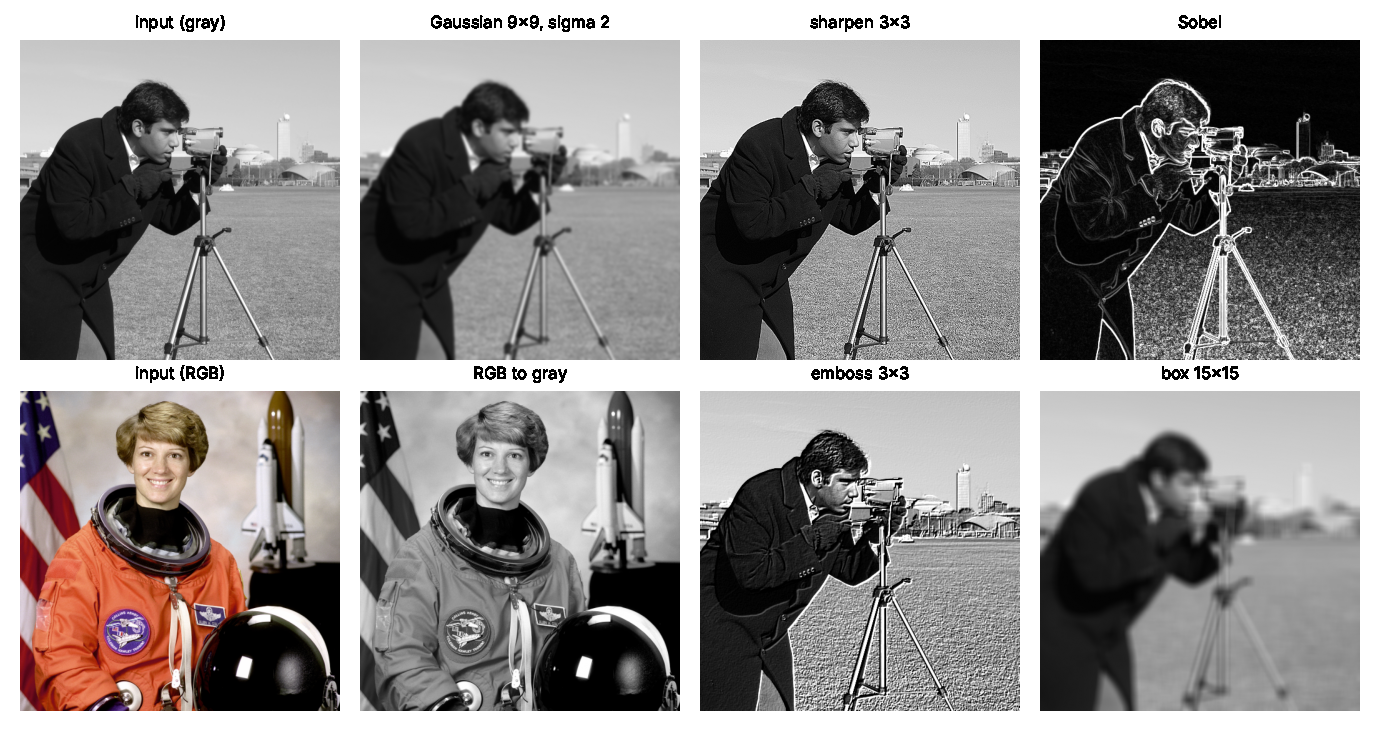
\includegraphics[width=\textwidth]{figures/f_ops_gallery.pdf}
\captionof{figure}{The operations on the standard ``cameraman'' photograph and on a colour image. Produced by the command line tool.}
\end{center}

\section{Sobel edge detection}

\subsection{The idea}

An edge is a place where brightness changes quickly. The change of brightness in a direction is a \emph{derivative}; for pixels it is the difference of neighbours. The simplest horizontal difference is $\text{in}(x+1)-\text{in}(x-1)$. Differences amplify noise, so Sobel first \emph{smooths} across the other direction using weights $1,2,1$ and only then differences:
\[
G_x=\begin{pmatrix}-1&0&1\\-2&0&2\\-1&0&1\end{pmatrix}\!*\text{in}
=\underbrace{\begin{pmatrix}1\\2\\1\end{pmatrix}}_{\text{smooth vertically}}\!\!\cdot\underbrace{\begin{pmatrix}-1&0&1\end{pmatrix}}_{\text{difference horizontally}}\!*\text{in},\qquad
G_y=\begin{pmatrix}-1&-2&-1\\0&0&0\\1&2&1\end{pmatrix}\!*\text{in}.
\]
$G_x$ responds to vertical edges, $G_y$ to horizontal edges. The edge strength combines both:
\begin{equation}
\text{out}=\min\!\big(255,\;|G_x|+|G_y|\big)\qquad\text{(the exact length would be }\sqrt{G_x^2+G_y^2}\text{)}.
\end{equation}
We use $|G_x|+|G_y|$, the common ``L1'' shortcut: it needs no square root, so it stays in integers and in 16-bit lanes. It overestimates the true length for diagonal edges by at most a factor $\sqrt2$, which is irrelevant for a detector that is thresholded afterwards, but you should know that it is an approximation.

\begin{center}
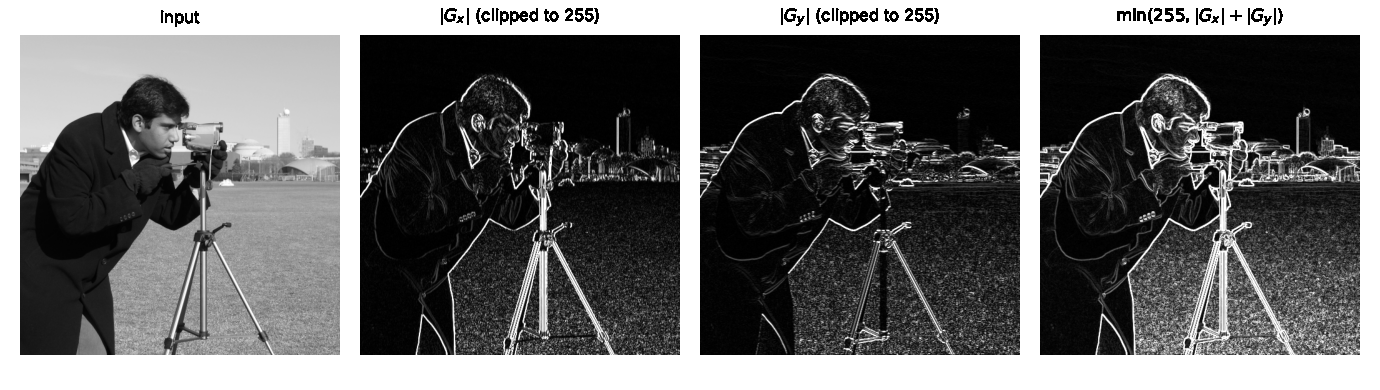
\includegraphics[width=\textwidth]{figures/f_sobel_parts.pdf}
\captionof{figure}{Left to right: the photograph, $|G_x|$ (vertical edges), $|G_y|$ (horizontal edges), and the final edge strength $\min(255,|G_x|+|G_y|)$.}
\end{center}

\subsection{How big can the numbers get? (this decides the data type)}

Each of $G_x$, $G_y$ is a sum of weights $\{1,2,1\}$ times pixels in $[0,255]$ with the positive and negative halves separated. The worst case is $4\cdot255=1020$ in magnitude, so $|G_x|+|G_y|\le2040<32\,768$. Everything fits in \textbf{signed 16-bit} integers (16 per 256-bit register) with no overflow: no wider type is needed, so no speed is wasted. Only the last step needs care: values above 255 must be clamped when converting back to 8 bits, which the instruction \code{packus} does for free (Chapter~\ref{ch:sobel}).

\begin{sound}
``Gray uses the 77/150/29 fixed-point weights, exact in 16-bit unsigned arithmetic, and I proved it for all 16.7 million colours. Sobel is the separable $[1\,2\,1]\otimes[-1\,0\,1]$ pair with an L1 magnitude, which stays within 16-bit signed lanes. Convolution is a $k\times k$ correlation in float32 with replicated borders and round-to-nearest-even output.''
\end{sound}

\chapter{The scalar versions, and what the compiler does by itself}\label{ch:scalar}

``Scalar'' means one number at a time: an ordinary loop. It is the baseline against which every speedup in this project is measured, so it must be (a) correct and (b) honest: not artificially slow.

\section{The structure shared by all versions}

Every implementation exposes the same three functions that compute only the output rows $y_0\dots y_1-1$:
\begin{lstlisting}
void rgbToGrayRows(const Image& src, Image& dst, int y0, int y1);
void sobelRows(const Image& src, Image& dst, int y0, int y1);
void convolveRows(const Image& src, Image& dst, const Kernel& k, int y0, int y1);
\end{lstlisting}
This tiny design decision pays for itself twice: OpenMP only has to hand each thread a range of rows (Chapter~\ref{ch:openmp}), and the tests can call the same row functions for any slice. The public functions in \file{dispatch.cpp} validate the arguments (sizes, channels, no overlap of source and destination, usable kernel) and then call the right implementation.

\section{Three levels of ``slow'': reference, scalar, autovec}

\begin{center}
\small
\begin{tabular}{@{}p{2.3cm}p{12.3cm}@{}}
\toprule
\textbf{reference} & Written for obviousness. Every pixel read goes through a helper that clamps the coordinates; Sobel is computed from the two $3\times3$ kernels literally; convolution is a double loop in float \emph{with an explicit fused multiply-add}, and a double-precision twin. Used only by the tests.\\
\textbf{scalar} & The code a careful programmer would write for speed: row pointers hoisted out of the loops, border pixels handled separately from the interior (so the interior has no clamping), \code{\_\_restrict} on pointers. Compiled with \code{-O3 -fno-tree-vectorize -fno-tree-slp-vectorize}: the auto-vectorizer is \textbf{off}.\\
\textbf{autovec} & Exactly the same source file, compiled with plain \code{-O3}: the auto-vectorizer is \textbf{on} (but with only the baseline instruction set, SSE2, unless you build with \code{-march=native}).\\ \bottomrule
\end{tabular}
\end{center}

\begin{plain}
\textbf{Why two builds of the same source?} The compiler can already turn some loops into SIMD loops. If you compare hand-written AVX2 only with a loop that the compiler was forbidden to vectorize you exaggerate your speedup. Comparing with an auto-vectorized build too tells the truth: how much did the compiler give you for free, and what did the hand-written intrinsics add on top? Both are in \file{src/scalar\_impl.inc}, \#included into two translation units with different flags (\file{Makefile}). Both use \code{-ffp-contract=off} so that \code{a*b+c} stays a multiply followed by an add and the two builds give identical bits.
\end{plain}

\section{The scalar code}

Three small helpers are shared by the loops: \code{clampInt} (limit an integer to a range, used for the replicated border), \code{sobelPixel} (the Sobel formula for one pixel, used for border pixels and tails by the AVX2 code too) and \code{roundClampF} (round-half-even and clamp to 0..255).

\lstinputlisting{snippets/code_scalar_helpers.cpp}

The row functions that use them:

\lstinputlisting{snippets/code_scalar_gray_sobel.cpp}

\lstinputlisting{snippets/code_scalar_conv.cpp}

Points worth mentioning in a review:
\begin{itemize}
\item In Sobel, \code{sobelPixel} gets the row pointers $y-1,y,y+1$ \emph{already clamped} at the top and bottom of the image, and the clamped column indices. The interior loop (\code{x = 1 \dots{} w-2}) passes \code{x-1,x,x+1} with no clamping.
\item In convolution the accumulation order is fixed: \code{j} (kernel row) outer, \code{i} (kernel column) inner. \textbf{This order is a contract.} All other versions use the same order for each output pixel, which is what makes them comparable bit for bit (Chapter~\ref{ch:numerics}).
\item \code{roundClampF} uses \code{lrintf}, which rounds to nearest, ties to even (the default CPU rounding mode), the same rule as the AVX2 instruction \code{cvtps2dq}.
\end{itemize}

\section{What did the auto-vectorizer do?}

The Makefile target \code{make vec-report} asks GCC to report every loop it vectorized in the auto-vectorized file (\code{-fopt-info-vec}). The result in this build:

\begin{center}\small\begin{tabular}{@{}p{5.6cm}p{3.2cm}p{3.2cm}p{3.6cm}@{}}\toprule
\textbf{loop} & \textbf{source line} & \textbf{vectorized by GCC?} & \textbf{reason if not}\\ \midrule
gray: loop over $x$ (3 interleaved channels) & scalar\_impl.inc:40 & no & failed \\
Sobel: interior loop over $x$ & scalar\_impl.inc:59 & \textbf{yes} (16-byte vectors) &  \\
convolution: loop over $x$ with the $k^2$ taps inside & scalar\_impl.inc:71 & no & loop nest containing two or more consecutive inner loops cannot be vec \\
convolution row-accumulate rewrite: \code{a[x] += wv * s[x]} & scalar\_autovec.cpp:38 & \textbf{yes} (16-byte vectors) &  \\
\bottomrule\end{tabular}\end{center}

\begin{plain}
\textbf{Why the natural convolution loop is not vectorized.} In the natural loop the $k^2$ taps of one output pixel are summed in the \emph{innermost} loops. There are two ways to use SIMD lanes on that: (a) vectorize the tap sum itself, which means adding the terms in a different order, and floating-point addition is not associative ($(a+b)+c\ne a+(b+c)$ in general), so GCC may not do it without \code{-ffast-math} (which also changes the results); or (b) vectorize over \emph{neighbouring pixels} (the outer $x$ loop), which keeps every pixel's order intact but requires vectorizing an outer loop that contains inner loops. For this loop nest the compiler's report says only ``loop nest containing two or more consecutive inner loops cannot be vectorized'' and fails the data-reference analysis of the inner loops; it does not say that associativity is the reason, and it would be wrong to claim so. What we can show by experiment: a programmer can restructure the loops so that pixels become the innermost dimension; \code{ablation::convolveAutoVecRowAcc} does that without changing a single bit of the result, GCC then vectorizes it, and Chapter~\ref{ch:bench} measures how far this gets compared with hand-written AVX2. Integer Sobel has no ordering problem and a simple loop, which is why GCC vectorizes it.
\end{plain}

\begin{sound}
``Scalar and autovec are the same source compiled with and without the vectorizer, so the comparison with intrinsics is fair. GCC vectorizes the integer Sobel loop but not the natural float convolution loop nest; restructuring the loops so pixels are the innermost dimension makes it vectorize, with identical result bits.''
\end{sound}

\chapter{Using all the cores: OpenMP}\label{ch:openmp}

\section{The idea}

A modern CPU has many cores, each able to run its own thread. Image filters are ideal for this: the output rows are independent of each other (an output pixel depends only on the \emph{input}, never on other output pixels), so rows can be computed in any order, on any core, at the same time. This kind of problem is called \emph{embarrassingly parallel} or \emph{data parallel}.

\textbf{OpenMP} is a standard way to tell the compiler ``run this block on several threads''. You write a \code{\#pragma} and the compiler and runtime (on GNU/Linux: \code{libgomp}) create and manage the threads.

\section{Our scheme: one contiguous band of rows per thread}

\lstinputlisting{snippets/code_omp_bands.cpp}

With $n$ threads the image is cut into $n$ horizontal bands of nearly equal height. Why \emph{contiguous bands} rather than letting each thread take single rows in turn (OpenMP's default \code{schedule(static,1)}-like interleaving)?
\begin{itemize}
\item \textbf{Locality.} Each thread streams through one contiguous block of memory, and its prefetcher can follow it. Neighbouring rows (needed by Sobel and convolution) are already in that thread's cache.
\item \textbf{No false sharing.} Threads write to different parts of the output; only a few cache lines at the band boundaries are shared, and only for reading the \emph{input}.
\item \textbf{Determinism.} The same thread count always gives the same split. And because each output pixel is computed from the input alone, using any number of threads gives \textbf{identical output}: the test \code{conv\_threads\_do\_not\_change\_the\_result} runs 1 to 200 threads and demands identical bits.
\end{itemize}
The price: if the work per row differs a lot, equal bands are unequal work (\emph{load imbalance}). For these kernels every row costs the same, so static bands are ideal; for irregular work you would use \code{schedule(dynamic)}.

\begin{plain}
\textbf{Edge cases handled on purpose.} If the number of threads exceeds the number of rows (the test uses 200 threads on 97 rows) some threads receive an empty band and simply do nothing. With \code{threads = 1} (or an image with a single row) no OpenMP region is started at all: the function is called directly, so the single-thread benchmarks contain no threading overhead. If the library is built without OpenMP (\code{make OPENMP=0}) the \code{threads} argument is ignored.
\end{plain}

\section{What limits the speedup?}

\begin{itemize}
\item \textbf{Amdahl's law.} If a fraction $s$ of the work cannot be parallelized, the speedup on $n$ threads is at most $1/(s+(1-s)/n)$. Here the serial parts are tiny (argument checks, thread start-up), so the limit is the next item.
\item \textbf{Memory bandwidth.} All cores share the path to main memory. A kernel that does very little arithmetic per byte (gray: 3 bytes in, 1 byte out, a few operations) can saturate the memory system with only a few threads; adding more cores then adds nothing. A kernel with a lot of arithmetic per byte (convolution with large $k$) keeps scaling. Chapter~\ref{ch:cache} quantifies this with a measured bandwidth yardstick.
\item \textbf{Thread start-up cost.} Creating or waking threads costs microseconds. For a tiny image this can exceed the work itself. (The benchmark's warm-up keeps the thread pool alive between calls.)
\item \textbf{CPU frequency and shared caches.} Running many cores can lower the clock speed and makes cores share the last-level cache.
\end{itemize}

\section{Controlling the threads from outside}

\begin{center}
\small
\begin{tabular}{@{}p{4.5cm}p{10.2cm}@{}}
\toprule
\code{OMP\_NUM\_THREADS=8} & Default thread count if the program does not ask. Our API always passes an explicit count.\\
\code{OMP\_PROC\_BIND=close} & Pin threads to cores and keep them adjacent; stops the operating system from moving them around between cores during a measurement.\\
\code{OMP\_PLACES=cores} & What a ``place'' is: one physical core (avoids using both hyper-threads of one core for two threads).\\
\code{taskset -c 0-7} / Slurm \code{--cpus-per-task} & Restrict the process to specific cores. On a Slurm node you get exactly the cores you asked for.\\ \bottomrule
\end{tabular}
\end{center}
The benchmark prints \code{OMP\_PROC\_BIND} and \code{OMP\_PLACES} at the top of its output so you can see how a measurement was made. The Slurm job scripts set them (Chapter~\ref{ch:cluster}).

\begin{warn}[First touch]
On a machine with several memory controllers (NUMA, e.g.\ two-socket nodes), a memory page lives near the core that first wrote to it. If one thread initializes the whole image and then many threads process it, some threads read ``remote'' memory, which is slower. Our \code{Image} constructor zeroes the buffer on the calling thread. For a single-socket benchmark with pinned threads this is fine; for a serious multi-socket study you would initialize the buffers in parallel with the same band split. This is a known limitation, worth stating if asked.
\end{warn}

\begin{sound}
``Each thread gets one contiguous band of output rows. Output pixels depend only on the input, so there is no synchronization and the result is bit-identical for every thread count, which my tests check from 1 to 200 threads. Scaling is limited by memory bandwidth for the low-arithmetic kernels, and I measured a copy bandwidth to show where the ceiling is.''
\end{sound}

\chapter{SIMD from zero: AVX2 in one chapter}\label{ch:simd}

\section{The idea}

\textbf{SIMD} means \emph{Single Instruction, Multiple Data}: one instruction operates on several numbers at once. Think of a checkout with one cashier scanning one item at a time (scalar) versus a conveyor that lets the cashier stamp 8 or 32 identical items with one press (SIMD).

Inside the CPU there are special wide registers. In \textbf{AVX2} they are \textbf{256 bits = 32 bytes} wide (named \code{ymm0}--\code{ymm15}). What is in the register is up to the instruction:

\begin{center}
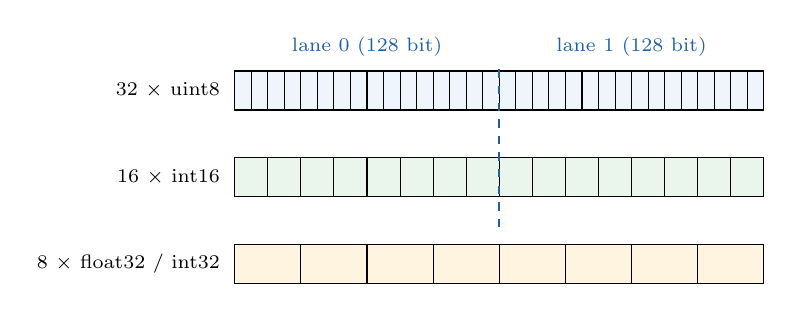
\begin{tikzpicture}[x=0.21cm,y=0.62cm,font=\tiny]
\draw[fill=plainbg] (0,0) rectangle (32,0.8);
\foreach \i in {0,...,31} {\draw (\i,0) -- (\i,0.8); }
\node[anchor=east,font=\scriptsize] at (-0.3,0.4) {32 $\times$ uint8};
\begin{scope}[yshift=-1.1cm]
\draw[fill=soundbg] (0,0) rectangle (32,0.8);
\foreach \i in {0,2,...,30} {\draw (\i,0) -- (\i,0.8); }
\node[anchor=east,font=\scriptsize] at (-0.3,0.4) {16 $\times$ int16};
\end{scope}
\begin{scope}[yshift=-2.2cm]
\draw[fill=warnbg] (0,0) rectangle (32,0.8);
\foreach \i in {0,4,...,28} {\draw (\i,0) -- (\i,0.8); }
\node[anchor=east,font=\scriptsize] at (-0.3,0.4) {8 $\times$ float32 / int32};
\end{scope}
\draw[dashed,thick,accent] (16,-2.4) -- (16,1.0);
\node[font=\scriptsize,accent] at (8,1.3) {lane 0 (128 bit)};
\node[font=\scriptsize,accent] at (24,1.3) {lane 1 (128 bit)};
\end{tikzpicture}
\end{center}
The same 256 bits can be read as 32 bytes, 16 half-words, or 8 floats. One \code{vaddps} adds 8 pairs of floats; one \code{vpaddw} adds 16 pairs of 16-bit integers. Peak throughput therefore goes up by 8 to 32 times for the same number of instructions, \emph{if} the data is arranged so that the lanes do useful, independent work.

\section{Reading an intrinsic's name}

You write SIMD code in C++ with \textbf{intrinsics}: functions (declared in \code{<immintrin.h>}) that the compiler turns into one machine instruction each. The names follow a pattern:
\[
\texttt{\_mm256\_add\_epi16}\;=\;\underbrace{\texttt{\_mm256}}_{\text{256-bit register}}\;\underbrace{\texttt{add}}_{\text{operation}}\;\underbrace{\texttt{epi16}}_{\text{16-bit signed int elements}}
\]
Type suffixes: \code{epi8/16/32/64} signed integers, \code{epu8/16} unsigned, \code{ps} packed single-precision floats, \code{si256} ``whole register, no element meaning''. \code{\_mm\_} (no number) means 128-bit. The C++ types are \code{\_\_m256} (8 floats), \code{\_\_m256i} (integers of any width), \code{\_\_m128i}.

\section{Every instruction this project uses}

\begin{center}
\small
\begin{tabular}{@{}p{5.2cm}p{9.4cm}@{}}
\toprule
\textbf{intrinsic} & \textbf{what it does}\\ \midrule
\code{\_mm\_loadu\_si128} / \code{\_mm\_storeu\_si128} & load / store 16 bytes from / to \emph{any} address (``u'' = unaligned allowed).\\
\code{\_mm256\_loadu\_ps}, \code{\_mm256\_storeu\_si256} & the same for 8 floats / 32 bytes.\\
\code{\_mm\_shuffle\_epi8} (\code{pshufb}) & for each output byte, pick the input byte named by an index (inside one 128-bit register); an index with the top bit set writes 0. The deinterleaving tool of Chapter~\ref{ch:gray}.\\
\code{\_mm256\_cvtepu8\_epi16} & \emph{widen}: 16 bytes $\to$ 16 unsigned 16-bit numbers (zero-extend). \code{cvtepu8\_epi32}: 8 bytes $\to$ 8 int32.\\
\code{\_mm256\_add/sub/mullo\_epi16} & 16 additions / subtractions / low 16 bits of products, at once.\\
\code{\_mm256\_abs\_epi16}, \code{\_mm256\_srli\_epi16} & absolute value; logical shift right of each 16-bit element.\\
\code{\_mm256\_packus\_epi16} & \emph{narrow with saturation}: two registers of int16 $\to$ one of uint8, clamping each value into $[0,255]$.\\
\code{\_mm256\_packs\_epi32} & narrow int32 $\to$ int16 with signed saturation.\\
\code{\_mm256\_permute4x64\_epi64}, \code{\_mm256\_permutevar8x32\_epi32} & move 64-bit or 32-bit pieces \emph{across} the two 128-bit halves (needed after the packs, see below).\\
\code{\_mm256\_cvtepi32\_ps} / \code{\_mm256\_cvtps\_epi32} & int32 $\leftrightarrow$ float32; the float $\to$ int conversion rounds to nearest even.\\
\code{\_mm256\_broadcast\_ss} & copy one float into all 8 lanes (used for the filter weight).\\
\code{\_mm256\_fmadd\_ps}$(a,b,c)$ & $a\cdot b+c$ for 8 floats, with a \emph{single} rounding (fused multiply-add, from the FMA3 extension).\\ \bottomrule
\end{tabular}
\end{center}

\section{Two things that trip everyone up}

\subsection{Lanes: the 256-bit register is really two 128-bit halves}

Most AVX2 integer instructions work inside each 128-bit half separately. \code{packus}, for example, packs the \emph{low half of both inputs} into the low half of the output and the high halves into the high half, so the output order is scrambled relative to the input order. A \emph{permute} afterwards puts the pixels back in order. Chapters~\ref{ch:sobel} and \ref{ch:conv} show the exact pictures; the unit tests catch any slip because the result would be garbled.

\subsection{Tails: the image width is rarely a multiple of the vector width}

A loop that handles 16 pixels per step ends with 0--15 pixels left. Options: pad the image (needs control over the input), a masked store, or handle the remainder with scalar code. We use scalar code for gray/Sobel remainders and a small temporary buffer for convolution. The tests use widths $1,2,3,\dots,15,16,17,\dots,129$ \emph{because} every width class near 16, 32 and 64 has a different tail length.

\section{Compiling and calling it safely}

\begin{itemize}
\item AVX2 and FMA instructions only exist on CPUs from about 2013/2014 on. Compiling a file with \code{-mavx2 -mfma} lets the compiler emit them \emph{anywhere} in that file. We therefore compile \textbf{only} \file{avx2.cpp} with those flags, and call into it \textbf{only after} a run-time CPU check (\code{\_\_builtin\_cpu\_supports("avx2")}) in \file{dispatch.cpp}. The rest of the library runs on any x86-64 CPU.
\item A global object with a constructor in \file{avx2.cpp} would execute at program start, before any check, and could crash an old CPU. The shuffle masks are therefore \code{constexpr} tables, computed by the compiler.
\item Alternative: compile everything with \code{-march=native}. Simpler and often slightly faster, but the binary may crash with ``illegal instruction'' on a different CPU model. On a cluster with several node types that is a real risk, so the Slurm scripts build per node type.
\end{itemize}

\begin{sound}
``AVX2 gives 256-bit registers: 32 bytes, 16 words or 8 floats. I compile only the intrinsics file with \code{-mavx2 -mfma} and gate it with a run-time CPU check. The two details I had to design around were the 128-bit lane structure (packs scramble the order, so I permute afterwards) and tails (scalar remainder, or a temporary buffer so nothing is ever written past the row).''
\end{sound}

\chapter{AVX2 grayscale, line by line}\label{ch:gray}

Reminder: $Y=(77R+150G+29B+128)\gg8$. The scalar code does this for one pixel per loop iteration. The AVX2 code converts \textbf{16 pixels per iteration}.

\section{Problem 1: the three channels are interleaved}

Memory contains \code{R0 G0 B0 R1 G1 B1 R2 \dots}. To multiply all red values by 77 with one instruction we need 16 reds next to each other in a register, and likewise for green and blue. Getting from the interleaved layout to three separate registers is called \emph{deinterleaving}.

Sixteen pixels are 48 bytes: exactly three 16-byte loads. Call them $v_0$ (bytes 0--15), $v_1$ (bytes 16--31) and $v_2$ (bytes 32--47).

\begin{center}
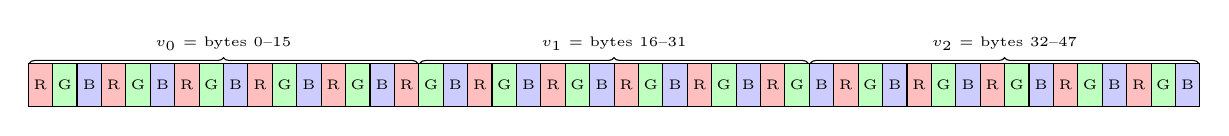
\begin{tikzpicture}[x=0.31cm,y=0.7cm,font=\tiny]
\foreach \i in {0,...,47} {
  \pgfmathtruncatemacro{\c}{mod(\i,3)}
  \pgfmathtruncatemacro{\p}{int(\i/3)}
  \node[draw,minimum width=0.31cm,minimum height=0.55cm,inner sep=0,
        fill=\ifcase\c red!25\or green!25\else blue!20\fi] at (\i,0) {\ifcase\c R\or G\or B\fi};
}
\foreach \k in {0,1,2} {
  \draw[decorate,decoration={brace,amplitude=2pt}] (16*\k-0.45,0.4) -- node[above=1pt]{$v_{\k}$ = bytes \the\numexpr16*\k\relax--\the\numexpr16*\k+15\relax} (16*\k+15.45,0.4);
}
\end{tikzpicture}
\end{center}

The reds are at byte positions $0,3,6,\dots,45$: six of them in $v_0$, five in $v_1$, five in $v_2$. \code{pshufb} (\code{\_mm\_shuffle\_epi8}) takes a register of data and a register of \emph{indices}: output byte $i$ is the data byte whose number is given in the index byte $i$; an index with its top bit set (we use \code{0x80}) produces a zero byte. So for each colour we build three index vectors, one per source register, which collect that colour's bytes into their final positions and leave zeros elsewhere. OR-ing the three partial results gives all 16 values of that colour in order.

\begin{center}
\small
\begin{tabular}{@{}cccc@{}}\toprule
 & mask for $v_0$ & mask for $v_1$ & mask for $v_2$\\ \midrule
\textbf{R} & \texttt{ 0  3  6  9 12 15 -- -- -- -- -- -- -- -- -- --} & \texttt{-- -- -- -- -- --  2  5  8 11 14 -- -- -- -- --} & \texttt{-- -- -- -- -- -- -- -- -- -- --  1  4  7 10 13} \\
\textbf{G} & \texttt{ 1  4  7 10 13 -- -- -- -- -- -- -- -- -- -- --} & \texttt{-- -- -- -- --  0  3  6  9 12 15 -- -- -- -- --} & \texttt{-- -- -- -- -- -- -- -- -- -- --  2  5  8 11 14} \\
\textbf{B} & \texttt{ 2  5  8 11 14 -- -- -- -- -- -- -- -- -- -- --} & \texttt{-- -- -- -- --  1  4  7 10 13 -- -- -- -- -- --} & \texttt{-- -- -- -- -- -- -- -- -- --  0  3  6  9 12 15} \\
\bottomrule\end{tabular}

{\footnotesize output byte $i$ = input byte at the listed index; \texttt{--} means index \texttt{0x80} (write 0)}
\end{center}

The tables are built by the compiler at compile time from one formula: pixel $i$'s colour-$c$ byte sits at global position $g=3i+c$, so it is read from source register $\lfloor g/16\rfloor$ at index $g\bmod16$.

\lstinputlisting{snippets/code_avx2_masks.cpp}

\section{Problem 2: the arithmetic must not overflow}

After deinterleaving, each colour is 16 bytes. We widen them to 16-bit lanes (\code{cvtepu8\_epi16}), multiply by 77, 150, 29 (\code{mullo\_epi16}, keeps the low 16 bits of each product) and add (with the $+128$). We showed in Chapter~\ref{ch:math} that the largest value is $65\,408<65\,536$: no wrap-around, so the low 16 bits of the products are the full products and plain 16-bit adds are exact. The shift \code{srli\_epi16(\dots,8)} divides by 256; it is a \emph{logical} shift, which is right because the values are unsigned.

\section{Problem 3: narrowing back to bytes}

The 16 results are 16-bit values in $[0,255]$ in one 256-bit register. \code{packus\_epi16} of the low and high 128-bit halves produces one 16-byte register in the original order, which is stored with one \code{storeu}.

\section{The complete kernel}

\lstinputlisting{snippets/code_avx2_gray.cpp}

\begin{plain}
\textbf{The tail.} The loop condition \code{x + 16 <= w} guarantees that the three loads (which read bytes $3x\dots3x+47$) stay inside the row: row $y$ has $3w$ bytes and the last pixel read is $x+15\le w-1$. The remaining 0--15 pixels use the scalar formula. Because the test suite uses \emph{tight} images (stride equal to the row size and an allocation that ends exactly after the last row), AddressSanitizer would flag a load one byte too far.
\end{plain}

\section{Why this is only a few times faster, not 16 times}

Per 16 pixels the code issues 3 loads, 9 shuffles, 6 ORs, 3 widenings, 3 multiplies, 4 adds, 1 shift, 1 pack and 1 store: about 30 instructions, around 2 per pixel, compared with about 10 per pixel for scalar code. The speedup is therefore roughly 5$\times$ in the instruction count, and then memory starts to limit: the kernel reads 3 bytes and writes 1 byte per pixel and has very little arithmetic to hide the memory traffic. Chapter~\ref{ch:cache} puts a number on how close it gets to the memory ceiling.

\begin{sound}
``For gray I deinterleave 16 pixels with nine \code{pshufb} shuffles using constexpr index tables, widen to 16-bit, do the three multiplies and the rounding add in 16-bit lanes (the maximum is 65{,}408, so no overflow), shift, and pack back. I verified it against all 16.7 million RGB colours. It is a memory-heavy kernel, so I compared its throughput with a memory-copy yardstick.''
\end{sound}

\chapter{AVX2 Sobel, line by line}\label{ch:sobel}

Recall: $G_x=(a_2-a_0)+2(b_2-b_0)+(c_2-c_0)$ and $G_y=(c_0+2c_1+c_2)-(a_0+2a_1+a_2)$, where $a,b,c$ are the rows above, at and below the pixel, and the index $0,1,2$ means column $x-1,x,x+1$.

\section{Vectorizing across pixels}

For one pixel this needs 8 neighbours. For 16 \emph{adjacent} pixels it needs 16-byte loads from each of the three rows at three column offsets: $x-1$, $x$ and $x+1$. Because loads may start at any address, ``the same row shifted by one pixel'' is just another load. That is the key trick of SIMD filtering: instead of shuffling data inside registers, load the row three times at three offsets.

\begin{center}
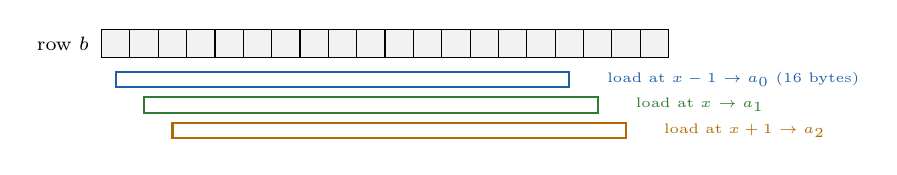
\begin{tikzpicture}[x=0.36cm,y=0.65cm,font=\scriptsize]
\foreach \i in {0,...,19} {\node[draw,minimum size=0.36cm,inner sep=0,fill=gray!10] at (\i,0) {};}
\node[anchor=east] at (-0.6,0) {row $b$};
\draw[thick,accent] (0.5-0.5,-0.55) rectangle (16.5-0.5+0,-0.85+0.0);
\node[font=\tiny,accent,anchor=west] at (17,-0.70) {load at $x-1$ $\to a_0$ (16 bytes)};
\draw[thick,soundfg] (1.5-0.5,-1.05) rectangle (17.5-0.5,-1.35);
\node[font=\tiny,soundfg,anchor=west] at (18,-1.20) {load at $x$ $\to a_1$};
\draw[thick,warnfg] (2.5-0.5,-1.55) rectangle (18.5-0.5,-1.85);
\node[font=\tiny,warnfg,anchor=west] at (19,-1.70) {load at $x+1$ $\to a_2$};
\end{tikzpicture}
\end{center}

Each loaded byte vector is widened to sixteen 16-bit numbers (\code{cvtepu8\_epi16} straight from memory), because the sums exceed 255. The row in the middle ($b$) needs only $b_0$ and $b_2$ (its centre pixel has weight 0 in $G_x$ and in $G_y$): 8 loads per 16 pixels.

\section{The arithmetic in 16-bit lanes}

\begin{enumerate}
\item $G_x=(a_2-a_0)+(c_2-c_0)+2(b_2-b_0)$; doubling is an addition of the value to itself.
\item $G_y=(c_0+c_2+2c_1)-(a_0+a_2+2a_1)$.
\item $m=|G_x|+|G_y|$ with \code{abs\_epi16} and \code{add\_epi16}.
\end{enumerate}
All of these fit in signed 16-bit: $|G_x|,|G_y|\le1020$ and $m\le2040$ (Chapter~\ref{ch:math}).

\section{Clamping and packing for free}

\code{packus\_epi16} converts int16 to uint8 \emph{with saturation}: negative values would become 0 and values above 255 become 255. Since $m\ge0$, the result is exactly $\min(m,255)$: the clamp of the formula costs no extra instruction.

But \code{packus} works separately inside the two 128-bit lanes:
\begin{center}
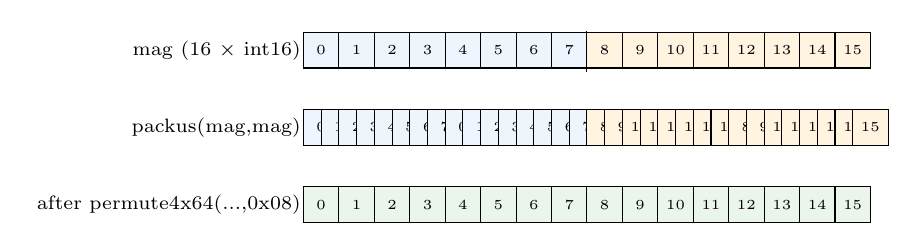
\begin{tikzpicture}[x=0.45cm,y=0.7cm,font=\tiny]
\node[anchor=east,font=\scriptsize] at (-0.3,1.6) {\code{mag} (16 $\times$ int16)};
\foreach \i in {0,...,15} {\node[draw,minimum size=0.45cm,inner sep=0,fill=\ifnum\i<8 plainbg\else warnbg\fi] at (\i,1.6) {\i};}
\draw[dashed] (7.5,1.2) -- (7.5,2.0);
\node[anchor=east,font=\scriptsize] at (-0.3,0.2) {\code{packus(mag,mag)}};
\foreach \i/\v in {0/0,1/1,2/2,3/3,4/4,5/5,6/6,7/7,8/0,9/1,10/2,11/3,12/4,13/5,14/6,15/7,16/8,17/9,18/10,19/11,20/12,21/13,22/14,23/15,24/8,25/9,26/10,27/11,28/12,29/13,30/14,31/15} {
  \node[draw,minimum size=0.45cm,inner sep=0,fill=\ifnum\i<16 plainbg\else warnbg\fi] at (\i*0.5,0.2) {\v};}
\node[anchor=east,font=\scriptsize] at (-0.3,-1.2) {after \code{permute4x64(...,0x08)}};
\foreach \i/\v in {0/0,1/1,2/2,3/3,4/4,5/5,6/6,7/7,8/8,9/9,10/10,11/11,12/12,13/13,14/14,15/15} {
  \node[draw,minimum size=0.45cm,inner sep=0,fill=soundbg] at (\i,-1.2) {\v};}
\end{tikzpicture}
\end{center}
The upper picture shows which pixel each byte holds. After \code{packus(mag,mag)} the low lane holds pixels $0..7$ twice and the high lane pixels $8..15$ twice (as 64-bit groups: $[0..7],[0..7],[8..15],[8..15]$). \code{permute4x64} with immediate \code{0x08} selects 64-bit group 0 and group 2 into the low 128 bits: pixels $0..15$ in order. One 16-byte store writes them.

\section{The complete kernel}

\lstinputlisting{snippets/code_avx2_sobel.cpp}

\begin{plain}
\textbf{Borders and tails.} Rows above the first and below the last are handled by pointing the row pointers at the first/last row (replication), so the vector loop needs no special case in $y$. In $x$: pixel 0 and pixel $w-1$ need clamped column indices, so they are computed by the scalar helper; the vector loop runs over $x=1,17,33,\dots$ as long as its widest load ($x+16$) stays within the row ($x+16\le w-1$); the rest uses the scalar helper. A tempting off-by-one (\code{x + 16 <= w}) would let the last vector read one byte beyond the row \emph{and be silently corrected} by the scalar write of the last pixel. Only the sanitizer build catches that kind of bug, which is why the test suite includes images with no padding and the \code{make asan-test} target (Chapter~\ref{ch:testing}).
\end{plain}

\begin{sound}
``Sobel is vectorized across 16 adjacent pixels with unaligned loads of each row at offsets $-1,0,+1$, 16-bit signed arithmetic (the maximum is 2040), absolute values, and \code{packus} which gives the clamp to 255 for free. \code{packus} works per 128-bit lane, so a \code{permute4x64} restores pixel order. The borders and the tail use the scalar helper, and I check that no vector load goes past the end of the row with AddressSanitizer on images with no padding.''
\end{sound}

\chapter{AVX2 convolution, line by line}\label{ch:conv}

Convolution is where AVX2 pays off the most: lots of arithmetic per pixel ($2k^2$ floating-point operations) and a very regular pattern. There are four ideas in the kernel.

\section{Idea 1: convert each row to float once, with the border built in}

The arithmetic is done in float32, but the image is bytes. Converting a byte to a float for every tap (every multiplication) would waste time: a pixel is used $k^2$ times. Instead, for each source row we create \emph{one padded float copy}:
\[
\text{padded}[j]=\text{src}[\operatorname{clamp}(j-r,\,0,\,w-1)],\qquad j=0,\dots,\text{round}_{64}(w)+2r-1 .
\]
The $r$ extra entries on each side replicate the edge pixel, so the \textbf{border handling disappears from the inner loop}: every output pixel, even the first, reads $k$ consecutive floats from the padded row. Extra entries beyond the right border let the vector loop run in full blocks of 64 pixels.

\lstinputlisting{snippets/code_avx2_convert_row.cpp}

\section{Idea 2: a ring of $k$ float rows, each converted only once}

Output row $y$ needs source rows $y-r\dots y+r$ ($k$ rows). Output row $y+1$ needs $y-r+1\dots y+r+1$: only \emph{one new row}. The code keeps $k$ padded rows in a small cache (slots); when moving to the next output row it converts just the one new source row into a free slot, and re-uses the rest. At the top and bottom of the image the clamped row indices repeat (row 0 is needed several times); the slot lookup by \emph{source row number} handles this without special cases.

\begin{center}
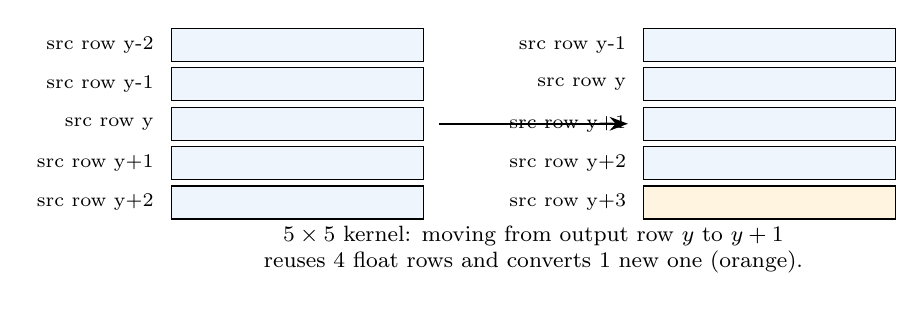
\begin{tikzpicture}[x=1cm,y=0.5cm,font=\scriptsize]
\foreach \i/\t in {0/{y-2},1/{y-1},2/{y},3/{y+1},4/{y+2}} {
  \node[draw,minimum width=3.2cm,minimum height=0.42cm,fill=plainbg] at (1.8,-\i) {};
  \node[anchor=east] at (0.1,-\i) {src row \t};}
\foreach \i/\t in {0/{y-1},1/{y},2/{y+1},3/{y+2}} {
  \node[draw,minimum width=3.2cm,minimum height=0.42cm,fill=plainbg] at (7.8,-\i) {};
  \node[anchor=east] at (6.1,-\i) {src row \t};}
\node[draw,minimum width=3.2cm,minimum height=0.42cm,fill=warnbg] at (7.8,-4) {};
\node[anchor=east] at (6.1,-4) {src row y+3};
\node[font=\footnotesize,align=center] at (4.8,-5.2) {$5\times5$ kernel: moving from output row $y$ to $y+1$\\reuses 4 float rows and converts 1 new one (orange).};
\draw[-{Stealth},thick] (3.6,-2) -- (6.0,-2);
\end{tikzpicture}
\end{center}

Working set: $k$ rows of $(w+2r)$ floats. For $w=4096$ and $k=9$ that is $9\cdot4104\cdot4$ bytes $\approx 148$\,KB, which fits in the L2 cache of the CPUs we use (Chapter~\ref{ch:cache}). This is the \textbf{cache-aware} part of the design: the image is streamed once from memory, and everything that is re-used lives in the cache.

\section{Idea 3: eight accumulators in registers, one broadcast weight}

For a block of 64 adjacent output pixels (8 vectors of 8 floats) the kernel keeps \textbf{8 accumulators in registers}, loops over the $k^2$ taps, and for each tap does
\[
\text{acc}_v \mathrel{+}= w_{ji}\cdot \text{padded}_j[x+i+8v],\qquad v=0,\dots,7,
\]
using \code{broadcast\_ss} to copy the weight into all lanes and \code{fmadd\_ps} to multiply-add. The loads at offset $+i$ are, again, plain unaligned loads of the same row shifted by one float.

Why 8 accumulators? An FMA has a \emph{latency} of about 4 cycles (the result is not ready for 4 cycles) but a modern core can \emph{start} two per cycle. If each FMA depends on the previous one (a single accumulator), the core waits 4 cycles for each; with 8 independent accumulators it can keep both FMA units busy. The ablation with 4 accumulators measures the difference (Chapter~\ref{ch:bench}).

\begin{plain}
\textbf{Registers vs.\ memory.} Because the accumulators stay in registers for all $k^2$ taps, the only memory traffic in the inner loop is reading the padded rows (served by the cache). The alternative that a compiler can produce from the ``row accumulate'' loop nest, \code{acc[x] += w * row[x+i]} over a whole row, reads and writes the accumulator array in memory for \emph{every} tap. \code{ablation::convolveAutoVecRowAcc} is exactly that, and the measured gap to the register version is large.
\end{plain}

\section{Idea 4: the same order of operations as the scalar code}

Every output pixel is accumulated starting from 0, with taps in the order $j=0,\dots,k-1$ (outer) and $i=0,\dots,k-1$ (inner). The vector code does the same for its 64 pixels in parallel; vectorizing across pixels changes which pixels are computed together, but never the order of operations \emph{within} one pixel. As a result:
\begin{itemize}
\item AVX2 is bit-identical to a scalar \code{fmaf} loop in the same order (the reference), for every kernel and image: tested.
\item The scalar and autovec versions are bit-identical to each other (multiply, then add).
\item Differences between the two families are possible only because one fuses the multiply-add (one rounding) and the other does not (two roundings). Chapter~\ref{ch:numerics} analyses that.
\end{itemize}

\section{Converting back to bytes}

After the taps, each accumulator holds 8 float sums. \code{cvtps\_epi32} rounds them to nearest, ties to even (the CPU's default mode, the same rule as the scalar \code{lrintf}); \code{packs\_epi32} narrows int32 to int16 and \code{packus\_epi16} narrows to uint8, \emph{both with saturation}, which implements the clamp to $[0,255]$. As in the Sobel kernel the two-lane structure scrambles the order, here in units of 4 pixels; one \code{permutevar8x32} with the index vector $(0,4,1,5,2,6,3,7)$ restores it:

\begin{center}
\small
\begin{tabular}{@{}lcccccccc@{}}
\toprule
after \code{packus}, 32-bit group: & 0 & 1 & 2 & 3 & 4 & 5 & 6 & 7\\
contains pixels: & 0--3 & 8--11 & 16--19 & 24--27 & 4--7 & 12--15 & 20--23 & 28--31\\ \midrule
index vector picks group: & 0 & 4 & 1 & 5 & 2 & 6 & 3 & 7\\
so the output contains pixels: & 0--3 & 4--7 & 8--11 & 12--15 & 16--19 & 20--23 & 24--27 & 28--31\\ \bottomrule
\end{tabular}
\end{center}

\lstinputlisting{snippets/code_avx2_pack.cpp}

\section{The complete kernel}

\lstinputlisting{snippets/code_avx2_conv.cpp}

\begin{plain}
\textbf{The last block of a row.} If fewer than 64 pixels remain, the kernel still computes 64 pixels (the extra ones read replicated padding, which is defined data) but stores into a small temporary array and copies only the valid bytes (\code{memcpy(q + x, tmp, w - x)}). It never writes past the end of the row, which the padding test and the sanitizer check.

\textbf{Guard on the kernel weights.} \code{cvtps\_epi32} returns the value \code{0x80000000} for numbers outside the int32 range, which would turn a huge positive sum into 0 after the pack instead of 255. \code{Kernel::validate()} therefore rejects kernels with $255\sum|w|>10^9$ and non-finite weights, so scalar and AVX2 cannot diverge on overflow.
\end{plain}

\begin{sound}
``The AVX2 convolution converts each source row to a padded float row once, keeps $k$ of them in a small ring so the next output row reuses $k-1$ of them, and computes 64 output pixels per block with eight register accumulators and \code{fmadd}. Borders disappear because the padding is built into the row copy. Per pixel it accumulates in the same order as the scalar code, so it is bit-identical to an FMA reference; I tested that for 7 kernel sizes, widths around every block boundary, and several thread counts.''
\end{sound}

\chapter{Memory, caches and the roofline}\label{ch:cache}

Chapters~\ref{ch:gray}--\ref{ch:conv} made the arithmetic cheap. Once arithmetic is cheap, the question becomes: \emph{can the memory system deliver the pixels fast enough?} This chapter is the vocabulary and the measurements for that question.

\section{The memory hierarchy in one picture}

A CPU core cannot compute on data that is far away. Between the core and main memory (DRAM) sit small, fast memories called \textbf{caches}:

\begin{center}
\begin{tabular}{@{}lll@{}}
\toprule
level & typical size (per core / shared) & what it means for us\\
\midrule
registers & 16 vector registers of 32 bytes & the accumulators of the convolution live here\\
L1 data cache & tens of KB per core & a few image rows; latency of a few cycles\\
L2 cache & about 1--2 MB per core on current server CPUs & the $k$ float rows of the convolution ring\\
L3 cache & tens of MB, shared by the cores of a socket & small and medium images\\
main memory & many GB, shared & large images; the bandwidth is the limit\\
\bottomrule
\end{tabular}
\end{center}

The numbers differ per CPU. Never quote them from memory in an interview; print them with \code{lscpu} on the machine you measured on (the Slurm scripts store this in \file{meta.txt}). The sandbox used for the example numbers reports \texttt{L1d 96 KiB (2 instances), L2 4 MiB (2 instances)}, i.e.\ 48 KB and 2 MB per core, and a very large shared L3 that is a property of the virtual machine host. For the cluster partitions the bwHPC wiki lists the CPU types; the cache sizes of those models should be read from \code{lscpu} in your own job output rather than assumed.

Data moves between levels in \textbf{cache lines} of 64 bytes. Reading one byte brings in 64. This is why the library aligns rows to 64 bytes and why the vector loops are written to walk through memory in order: the \emph{hardware prefetcher} recognises a sequential stream and loads the next lines before the program asks for them.

\begin{plain}
\textbf{Library analogy.} The shelf next to your desk (L1) holds a few books. The room's shelves (L2/L3) hold many. The city library (DRAM) holds everything but every trip takes long. Good code reads a book once, uses everything in it, and puts it back. Bad code goes back to the library for every sentence.
\end{plain}

\section{Working sets of the three operations}

The \textbf{working set} is the data that is re-used before it is no longer needed.
\begin{itemize}
\item \textbf{Gray}: nothing is re-used. Each input byte is read once, each output byte written once. The working set is a few lines. It is a pure \emph{streaming} kernel: speed = how fast bytes flow.
\item \textbf{Sobel}: each source row is used by three consecutive output rows. The three rows are read in the same pass; the working set is three rows (a few KB to a few tens of KB, e.g.\ $3\cdot8192$ bytes). It fits in L1/L2 for any realistic width, so every source byte comes from DRAM \emph{once}. Streaming again.
\item \textbf{Convolution}: $k$ float rows of $w+2r$ entries, i.e.\ $4k(w+2r)$ bytes: 148 KB for $w=4096$, $k=9$ (Chapter~\ref{ch:conv}). That is bigger than L1 but fits in L2. The design keeps this ring in cache and streams the image once.
\end{itemize}

\section{Arithmetic intensity and the roofline}

Define the \textbf{arithmetic intensity} $I=\text{operations}/\text{bytes moved}$. A processor has two ceilings:
\[
\text{attainable performance}\;=\;\min\bigl(P_{\text{peak}},\;B\cdot I\bigr),
\]
where $P_{\text{peak}}$ is the peak arithmetic rate and $B$ the memory bandwidth. Plot performance against $I$: a sloped line on the left (memory-bound: more intensity is directly more speed) and a flat roof on the right (compute-bound). This is the \textbf{roofline model}.

\begin{itemize}
\item \textbf{Gray and Sobel} do a handful of integer operations per pixel and move 2--4 bytes per pixel: far left, memory-bound. Once SIMD has removed the instruction overhead, the next ceiling is the memory system.
\item \textbf{Convolution} does $2k^2$ floating-point operations per pixel for the same 2 bytes of traffic: $I=k^2$ operations per byte. Already for $k=3$ it is far to the right of the other two, so it is compute-bound and its limit is the FMA units.
\end{itemize}

\subsection{A measured memory yardstick}

To avoid guessing $B$, the benchmark has an operation \code{copy}: a multi-threaded \code{memcpy} of the same pixel rows into another image. A kernel cannot move bytes faster than a plain copy does, so its \emph{minimum traffic rate} (input bytes read plus output bytes written, counted once) should be compared with the copy's.

\begin{center}
\small
\begin{tabular}{@{}lrrrr@{}}
\toprule
image & threads & copy (GB/s) & gray AVX2 & Sobel AVX2\\
\midrule
2048$^2$ & 1 & 24.6 & 14.5 (59\,\%) & 8.0 (33\,\%) \\
2048$^2$ & 2 & 49.2 & 27.5 (56\,\%) & 15.6 (32\,\%) \\
4096$^2$ & 1 & 25.0 & 14.6 (58\,\%) & 8.4 (34\,\%) \\
4096$^2$ & 2 & 50.4 & 27.7 (55\,\%) & 16.3 (32\,\%)\\
\bottomrule
\end{tabular}
\end{center}


\begin{center}
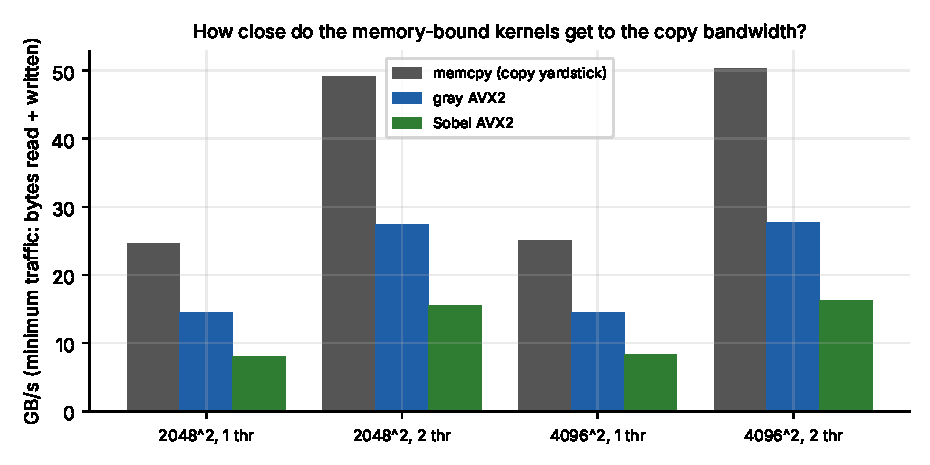
\includegraphics[width=0.85\textwidth]{figures/f_bandwidth.pdf}
\captionof{figure}{Minimum-traffic rate of the AVX2 kernels compared with a plain copy of the same pixels (sandbox VM).}
\end{center}

How to read this honestly:
\begin{itemize}
\item On this machine one thread copies about \copyOneBig\,GB/s from DRAM (images of 2048$^2$ and larger) and two threads about \copyTwoBig\,GB/s, so the sandbox did not saturate its memory with two threads. For small images that fit in cache the copy is faster (\copyOneSmall\,GB/s at 512$^2$), which is the cache hierarchy showing.
\item AVX2 gray reaches about \pctGrayOfCopy\,\% of the copy rate at 4096$^2$, Sobel about \pctSobelOfCopy\,\%. The copy rate counts a read and a write of one byte per pixel; gray reads three bytes per pixel and Sobel reads each pixel through three rows, so neither is expected to reach 100\,\% of that figure with a one-pass design. The conclusion is not ``at the roof'', it is: \emph{within a factor 2--3 of the memory ceiling}, which is where a SIMD kernel that does a little work per byte should be, and far from the instruction-bound regime of the scalar code.
\item This is a measurement on a VM. The same experiment on the cluster (E5 in the scripts) gives \emph{your} yardstick; a different number there is expected and fine.
\end{itemize}

\subsection{Compute side: how close is convolution to the FMA roof?}

The theoretical peak of one core with two 256-bit FMA units is $2\ \text{FMA}\times8\ \text{lanes}\times2\ \text{flop}=32$ flop/cycle. At the nominal 2.1\,GHz of the sandbox CPU that is \nominalPeakGf\,GFLOP/s, and the AVX2 convolution reaches up to \gfAvxMax\,GFLOP/s, about \fracOfNominalPeak\,\% of that figure. Two caveats keep this honest: (1) the clock under load may differ from the nominal value (turbo, or a lower AVX frequency), so the percentage is a rough indicator, not a precise efficiency; (2) the count $2k^2$ flop per pixel counts every tap as one multiply and one add, whether or not the zero weights could be skipped. What the number shows qualitatively: the kernel is limited by the FMA units, not by loads or by the memory system, which is exactly what the design of Chapter~\ref{ch:conv} aims for. Whether the cluster CPUs (Ice Lake, Zen 4) show the same fraction is a measurement for you to make; do not assume it.

\section{Image size and the cache}

\begin{center}
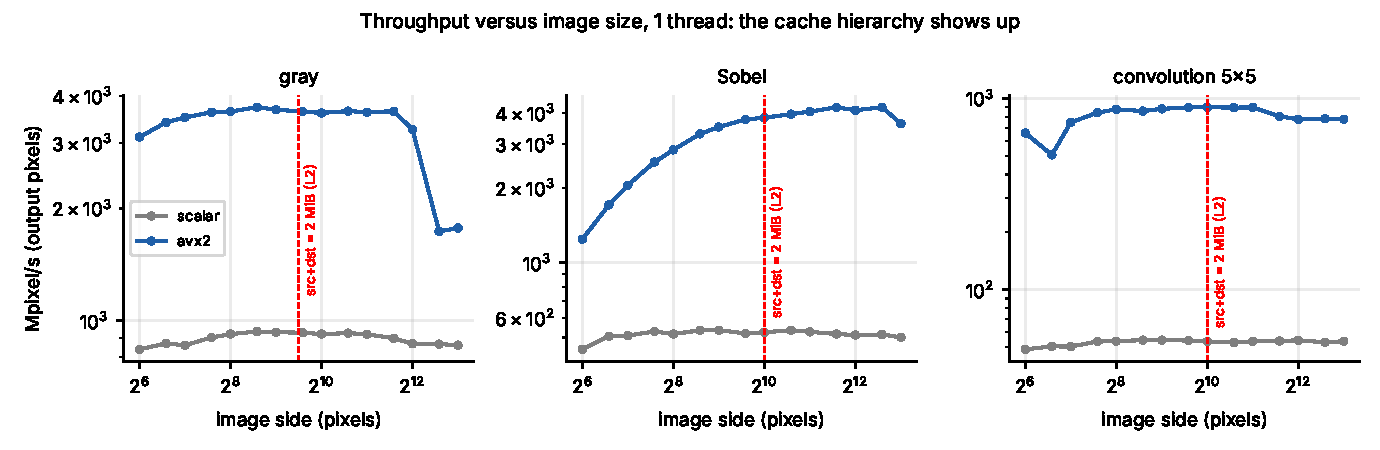
\includegraphics[width=\textwidth]{figures/f_sizes.pdf}
\captionof{figure}{Throughput of scalar and AVX2 versus image side (1 thread). The dashed red line marks the size at which source plus destination together (2 bytes per pixel, 4 for gray) equal 2 MiB, the per-core L2 of this VM.}
\end{center}

Observations in the sandbox data, with the explanation they support:
\begin{itemize}
\item \textbf{Scalar} throughput is flat: it is limited by instructions, and the memory system is never the bottleneck, so image size does not matter.
\item \textbf{AVX2 gray} falls from about \mpixGrayAvxSmall\,Mpix/s at 512$^2$ to about \mpixGrayAvxHuge\,Mpix/s at 8192$^2$ once the data come from DRAM: the SIMD kernel is fast enough to feel the memory.
\item \textbf{AVX2 Sobel} is much less sensitive (\mpixSobelAvxSmall to \mpixSobelAvxHuge\,Mpix/s): it does more arithmetic per byte, so it stays closer to compute-bound.
\item \textbf{Very small images} (below about 100 pixels per side) lose speed to fixed per-call costs: the vector loop only starts after the first pixel and ends before the last, so a larger share of pixels takes the scalar border path.
\end{itemize}

\section{Does the row stride matter?}

Chapter~\ref{ch:images} explained why the library avoids strides that are an exact multiple of 4096 bytes: addresses 4096 bytes apart map to the same cache set, so $k$ rows that are read together can evict each other (\emph{cache associativity conflict} and, on some CPUs, \emph{4K aliasing} between loads and stores). Sobel reads three rows and writes one at the same column offset: that is the pattern that would suffer.

The experiment compares the same operation with stride $=$ width (tight) and stride $=$ width $+64$. Strides of 4096 and 8192 bytes (widths 4096 and 8192) are exact page multiples; widths 1024 and 2048 are powers of two but not page multiples and serve as controls. The last six rows use a 4096-pixel-wide, 512-row image with large kernels.

\begin{center}
\small
\begin{tabular}{@{}llrrr@{}}
\toprule
width & case & stride = width (ms) & stride $+64$ (ms) & power-of-two slower by\\
\midrule
1024 & sobel scalar & 2.17 & 2.08 & +4.6\,\% \\
1024 & sobel avx2 & 0.28 & 0.28 & +0.1\,\% \\
1024 & conv avx2 k=9 & 3.30 & 3.28 & +0.6\,\% \\
2048 & sobel scalar & 8.60 & 8.99 & -4.3\,\% \\
2048 & sobel avx2 & 1.07 & 1.20 & -11.0\,\% \\
2048 & conv avx2 k=9 & 14.05 & 13.99 & +0.4\,\% \\
4096 & sobel scalar & 38.18 & 32.82 & +16.3\,\% \\
4096 & sobel avx2 & 4.40 & 3.99 & +10.4\,\% \\
4096 & conv avx2 k=9 & 56.25 & 55.43 & +1.5\,\% \\
8192 & sobel scalar & 137.21 & 130.16 & +5.4\,\% \\
8192 & sobel avx2 & 18.54 & 18.42 & +0.7\,\% \\
8192 & conv avx2 k=9 & 222.52 & 222.11 & +0.2\,\% \\
4096$\times$512 & conv scalar k=15 & 327.47 & 314.82 & +4.0\,\% \\
4096$\times$512 & conv autovec k=15 & 365.18 & 366.21 & -0.3\,\% \\
4096$\times$512 & conv avx2 k=15 & 17.44 & 17.49 & -0.3\,\% \\
4096$\times$512 & conv scalar k=21 & 680.57 & 637.85 & +6.7\,\% \\
4096$\times$512 & conv autovec k=21 & 693.49 & 699.34 & -0.8\,\% \\
4096$\times$512 & conv avx2 k=21 & 33.03 & 32.74 & +0.9\,\%\\
\bottomrule
\end{tabular}
\end{center}

\begin{center}
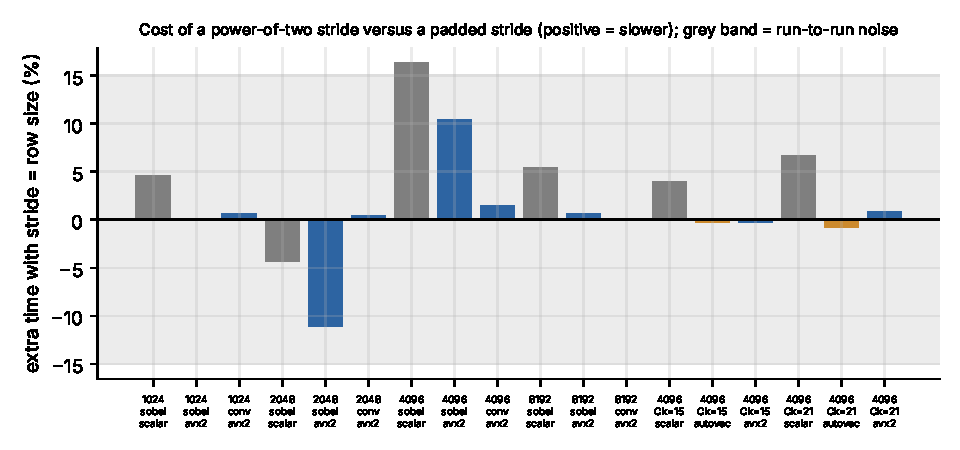
\includegraphics[width=0.95\textwidth]{figures/f_stride.pdf}
\captionof{figure}{Relative cost of the page-multiple stride. Positive values mean the padded stride is faster; the grey band is the run-to-run spread measured in E6 (at least $\pm5\,\%$).}
\end{center}

\begin{warn}[What this experiment does and does not show]
The effect is small and inconsistent: it ranges from about $\strideBestFast\,\%$ to $+\strideWorstSlow\,\%$ (positive: the page-multiple stride is slower), and the run-to-run spread on this VM is of the same order (Chapter~\ref{ch:bench}). The one result in the direction the theory predicts is Sobel at width 4096 (scalar $+16\,\%$, AVX2 $+10\,\%$); but width 8192, which is also a page multiple, shows only $+5\,\%$ and $+0.7\,\%$, width 2048 (not a page multiple) shows the \emph{opposite} sign, and convolution, whose working set is the float ring rather than the image rows, shows no effect beyond $\pm1.5\,\%$ for AVX2. So the honest statement is: \emph{``the padding costs 1.6\,\% memory and removes a failure mode that the theory predicts; on this VM I could not show an effect distinguishable from run-to-run noise.''} Do not claim a measured gain. Repeat E3 on the cluster (the script does), and report what you see, including a null result.
\end{warn}

\section{Other effects the code does not exploit (and you can mention)}

\begin{itemize}
\item \textbf{Tiling / loop blocking over several output rows} would let each loaded source row be used by more than one output row in registers (the convolution here reloads each float row once per output row that uses it: $k$ times). A $2\times$ or $4\times$ row blocking reduces loads; it is the next step toward the FMA roof.
\item \textbf{Non-temporal stores} (\code{\_mm256\_stream\_si256}) skip polluting the cache with output that will not be read again; they help bandwidth-bound writes of large images and hurt small ones.
\item \textbf{NUMA and first touch.} On a two-socket node, memory is attached to a socket. An image allocated and first written by one thread lives near that thread's socket; other sockets read it over a slower link. The scaling script pins threads close together to stay in one place. A full treatment would initialise the image in parallel with the same band layout (``first touch'').
\item \textbf{Huge pages} (2 MB) reduce the number of address translations (TLB misses) for large images.
\end{itemize}

\begin{sound}
``The three kernels sit at very different places on the roofline. Gray and Sobel stream: after vectorization their limit is memory bandwidth, and I measured how close they get with a memcpy of the same pixels. Convolution has $k^2$ operations per byte, so it is bound by the FMA units; the ring of float rows keeps the re-used data in L2, and I measured it at roughly \fracOfNominalPeak{} percent of the nominal peak of one core on my test machine \emph{[yours: on the cluster core]}.''
\end{sound}

\chapter{Numerics: what ``the same result'' means}\label{ch:numerics}

A SIMD library is only useful if its output can be trusted. This chapter defines exactly what is promised for each operation, and why the promise for convolution has to be stated more carefully than for the other two.

\section{Integer operations: exact}

Gray and Sobel use integers only. Integer addition and multiplication are exact as long as the numbers fit in the type; the proof that they fit is a short calculation (Chapter~\ref{ch:math}):
\begin{itemize}
\item gray: $77R+150G+29B+128\le255\cdot256+128=65\,408<2^{16}$, so unsigned 16-bit lanes never wrap. The test \code{gray\_exhaustive\_all\_16777216\_colours} does not rely on the proof alone: it feeds \emph{every one} of the $2^{24}$ possible colours through the AVX2, the scalar and the reference code and compares.
\item Sobel: $|G_x|,|G_y|\le1020$, $|G_x|+|G_y|\le2040<2^{15}$, so signed 16-bit lanes are enough.
\end{itemize}
Because there are no rounding errors, every implementation must give \textbf{identical bytes}, and every test of these two operations demands zero difference.

\section{Floating point in one page}

A 32-bit float stores a number as $\pm m\cdot2^{e}$ with a 24-bit significand $m$. Consequences:
\begin{itemize}
\item Not every number is representable: $0.1$ is not. Each arithmetic result is \textbf{rounded} to the nearest representable value. The relative error of one rounding is at most $u=2^{-24}\approx6\cdot10^{-8}$ (``unit roundoff'').
\item Addition is \textbf{not associative}: $(a+b)+c$ and $a+(b+c)$ can differ in the last bit. The order of the operations is part of the definition of the result.
\item A \textbf{fused multiply-add} (FMA) computes $a\cdot b+c$ with \emph{one} rounding instead of two. It is faster and slightly more accurate, but gives a \emph{different} last bit than multiply-then-add.
\end{itemize}

\begin{plain}
Think of rounding as measuring with a ruler that has a mark every millimetre. Add up a thousand lengths, rounding after every addition, and the total can be a millimetre or two off, and the \emph{size} of that error depends on the order in which you added. Nobody is wrong; the order is simply part of the recipe.
\end{plain}

\section{The convolution contract}

For one output pixel the library computes
\[
s=\sum_{j=0}^{k-1}\sum_{i=0}^{k-1}w_{ji}\,p_{ji},\qquad \text{out}=\operatorname{clamp}\bigl(\operatorname{rne}(s),0,255\bigr),
\]
with the summation order \textbf{fixed}: $j$ outer, $i$ inner, starting from $0$. ``rne'' is round to nearest, ties to even (the default IEEE mode: $0.5\to0$, $1.5\to2$, $2.5\to2$). Two families of implementations follow this recipe, differing in one thing only:

\begin{center}
\begin{tabular}{@{}lll@{}}
\toprule
family & each step is & produced by\\
\midrule
FMA family & $\text{acc}\leftarrow\operatorname{fma}(w,p,\text{acc})$ (one rounding) & AVX2 kernels and \code{reference::convolveFmaFloat}\\
two-rounding family & $\text{acc}\leftarrow\operatorname{fl}(\text{acc}+\operatorname{fl}(w\cdot p))$ & scalar, autovec, row-accumulate rewrite\\
\bottomrule
\end{tabular}
\end{center}

The build flags make this explicit: the scalar and autovec translation units are compiled with \code{-ffp-contract=off}, which forbids the compiler from silently turning multiply-add pairs into FMAs. Without that flag a build with \code{-march=native} would change the numerical results of ``scalar'' behind the programmer's back, and the claim ``these two are bit-identical'' would hold on one machine and fail on another.

What the tests then establish, in the order of strength:
\begin{enumerate}
\item \textbf{AVX2 $=$ FMA reference, bit for bit} (\code{conv\_avx2\_is\_bit\_identical\_to\_the\_fma\_reference}): the compared quantity is the output byte of every pixel for random kernels with positive and negative weights, many sizes, strides and thread counts. The reference is written independently with \code{fmaf} in the same order.
\item \textbf{scalar $=$ autovec $=$ row-accumulate rewrite, bit for bit}: same operations, same order, no FMA.
\item \textbf{Float32 versus exact arithmetic}: an implementation can differ from the exact result (computed in double precision, ties to even) only when the exact value lies so close to a rounding boundary ($x.5$) that the float rounding error moves it across. The test \code{conv\_scalar\_differs\_from\_exact\_rounding\_only\_next\_to\_ties} checks that every such difference occurs within the proven error bound of a tie, and never exceeds one grey level. The independent NumPy/SciPy cross-check (float64, Chapter~\ref{ch:testing}) measured \crossApproxPct\,\% of pixels differing by one grey level for box and Gaussian kernels over all three implementations, never by more. The FMA family and the two-rounding family can therefore differ from each other by one level on such near-ties; they cannot differ otherwise.
\item \textbf{Exact kernels, zero tolerance} (\code{conv\_binomial\_kernels\_are\_exact\_in\_every\_implementation}): for binomial kernels up to $9\times9$ the 2D weights are integer multiples of $2^{-16}$ at most, every product has fewer than 24 significant bits and every partial sum is a multiple of $2^{-16}$ below $2^{8}$, i.e.\ it needs at most $8+16=24$ bits. Nothing is ever rounded, the order does not matter, and \emph{all} implementations including the FMA family must agree exactly. This is the test that proves the data movement (shuffles, lane order, border logic) is right independently of any rounding argument.
\end{enumerate}

\section{An error bound that is tested, not just stated}

For a sum of $n=k^2$ terms in float arithmetic with FMA, the standard result is
\[
\bigl|\hat s-s\bigr|\;\le\;\gamma_n\sum|w_{ji}p_{ji}|\;\le\;\gamma_n\cdot255\sum|w_{ji}|,\qquad
\gamma_n=\frac{nu}{1-nu}.
\]
The test \code{conv\_float\_error\_is\_within\_the\_theoretical\_bound} computes the same sum in double precision (\code{reference::convolveDouble}, same order) and compares: the largest observed error was \errBoundRatio\ times the bound. In other words the bound holds with an order of magnitude to spare, as expected: it describes the worst case in which all rounding errors have the same sign and the largest size, which real data never does. In practice this means a float32 result has an error far below $\tfrac12$ grey level, and a mismatch in the output byte can occur only where the exact value is within about $10^{-4}$ of a rounding boundary.

\section{Rounding and clamping details that cause real bugs}

\begin{itemize}
\item \textbf{Round-half-even versus half-up.} The scalar code uses \code{lrintf}, the AVX2 code \code{cvtps\_epi32}; both use the processor's rounding mode (default: nearest-even). A kernel that rounds ``half up'' differs on every exact tie, so ties are not a theoretical curiosity: any kernel with power-of-two weights, such as the binomial filters, produces exact $x.5$ sums on integer pixels all the time. The mutation \emph{``truncate instead of round''} is killed by the tests.
\item \textbf{Clamp after rounding, not before.} A value of 255.4 must give 255, not 256 clamped later by wrap-around. The AVX2 path uses saturating packs (\code{packs\_epi32}, \code{packus\_epi16}), which clamp to $[-32768,32767]$ and then $[0,255]$. This is only correct if the 32-bit integer is itself correct, which needs the next point.
\item \textbf{Overflow in the float-to-int conversion.} \code{cvtps\_epi32} returns the ``integer indefinite'' value $-2^{31}$ for inputs outside the 32-bit range, which would turn a huge positive sum into the minimum and clamp it to 0, silently. \code{Kernel::validate} therefore rejects kernels where $255\sum|w|>10^9$ and any kernel containing NaN or infinity; the test \code{bad\_arguments\_are\_rejected} covers it.
\item \textbf{Negative weights.} Sharpening and emboss kernels produce negative sums; those clamp to 0. The test kernels include random weights in $[-1,1]$ so both clamp directions are exercised.
\item \textbf{The sum of the weights.} A blur must have $\sum w=1$ to preserve brightness; the Gaussian factory normalises in double and stores float. The test \code{conv\_blur\_of\_constant\_image\_is\_constant\_and\_brightness\_is\_kept} checks that a constant image stays constant.
\end{itemize}

\section{OpenCV and the 14-bit gray conversion}

OpenCV's \code{cvtColor} computes gray with 14-bit coefficients ($0.299,0.587,0.114$ scaled by $2^{14}$), the library with 8-bit coefficients ($77,150,29$ over 256). The results differ by up to 1 grey level on a minority of pixels (7.43\,\% on the test image). This is a \emph{design difference}, not a bug of either library, and Chapter~\ref{ch:bench} reports the comparison with that caveat. If an interviewer asks, the right statement is: ``8-bit coefficients keep the intermediate in 16 bits, so one 256-bit register processes 16 pixels; the price is a coefficient error of about $0.2\%$, and the output differs from the 14-bit conversion by at most one grey level.''

\begin{sound}
``For gray and Sobel the result is integer, so all implementations are bit-identical, and I checked the gray conversion for all 16.7 million colours. For convolution I fixed the accumulation order and compiled the scalar path with FMA contraction off. The AVX2 result equals an independent \code{fmaf} reference bit for bit; against a float64 SciPy reference a one-level difference occurs only on near-ties, in about seven of a million pixels for box and Gaussian kernels, and binomial kernels, which are exact in float, agree with zero tolerance. The float error stays below a tenth of the theoretical bound.''
\end{sound}

\chapter{Testing: how we know it is correct}\label{ch:testing}

Optimised code is dangerous in a specific way: it is full of tricks (shuffles, lane permutes, partial vectors, ring buffers), and a wrong trick often produces output that \emph{looks} right. A test suite for such code has to be designed against the failure modes of SIMD code, not just against ``does it run''. This chapter lists the layers, what each is for, and what the numbers mean.

\section{The layers}

\begin{center}
\small
\begin{tabularx}{\textwidth}{@{}>{\raggedright\arraybackslash}p{3.0cm}X@{}}
\toprule
layer & what it checks (and the test that does it)\\
\midrule
hand-computed examples & tiny images whose result a human can verify on paper: Sobel of a step edge, gray of primary colours. \emph{\code{gray\_known\_values}, \code{sobel\_hand\_computed\_examples}}\\
exhaustive & all $2^{24}$ colours through gray, no sampling. \emph{\code{gray\_exhaustive\_all\_16777216\_colours}}\\
properties & statements that follow from the maths and need no reference: Sobel of a constant image is 0; transposing the input transposes the output; inverting the input leaves the output unchanged; a delta kernel shifts the image; the identity kernel returns the input; blur keeps constants. \emph{\code{sobel\_symmetries\_hold}, \code{conv\_delta\_kernel\_shifts\_the\_image}, \dots}\\
reference equivalence & optimised versus a plain, obviously correct implementation over many sizes (22 widths from 1 to 129 chosen around the vector sizes 16, 32 and 64), strides, image contents and thread counts (1 to 8 for gray and Sobel; up to 200 in the dedicated thread test). \emph{the \code{\dots\_matches\_reference\_\dots} tests}\\
bit exactness & AVX2 $=$ FMA reference; scalar $=$ autovec; exact (binomial) kernels with zero tolerance. \emph{\code{conv\_avx2\_is\_bit\_identical\_to\_the\_fma\_reference}, \code{conv\_binomial\_kernels\_are\_exact\_in\_every\_implementation}}\\
numerical bound & observed float error versus the proven bound. \emph{\code{conv\_float\_error\_is\_within\_the\_theoretical\_bound}}\\
memory safety & images with no padding at all, run under AddressSanitizer; the padding bytes must be untouched. \emph{\code{tight\_images\_without\_any\_padding}, \code{outputs\_never\_touch\_the\_row\_padding}, \code{make asan-test}}\\
API contract & mismatched sizes, overlapping source and destination, even kernels and NaN weights must throw. \emph{\code{bad\_arguments\_are\_rejected}}\\
independent implementation & a second implementation by other libraries, in another language: NumPy and SciPy (and OpenCV where installed). \emph{\code{python/crosscheck.py}}\\
tests of the tests & seed one deliberate bug at a time and demand that the suite fails. \emph{\code{scripts/mutation\_test.sh}}\\
\bottomrule
\end{tabularx}
\end{center}

The suite has \testGroups\ test groups and executes \testChecks\ individual checks (a check is one comparison of a pixel, a size or a property); the last run reported \testFailures\ failures. The check count is dominated by the exhaustive gray test and the pixel-by-pixel comparisons; it is not a quality metric on its own, and the guide does not present it as one.

\section{Why the edge sizes matter most}

A vector loop processes $V$ pixels at a time (16 for gray and Sobel, 64 for the convolution block). The tail of the row, $w \bmod V$ pixels, is handled by a different code path. Almost all real SIMD bugs live in these paths: the last vector reads past the end, the tail is skipped, the block is partially written. So the tests are parameterised by width: a list of widths from 1 to 129 clustered around 16, 32, 64 (for example 15, 16, 17, 18, 19, 31, \dots, 65, 66), heights 1, 2, 3 and larger (the border logic in $y$ is different for images with fewer rows than the kernel), padded and unpadded strides.

\section{The memory-safety trap: a bug the output cannot show}

Consider this bug in the Sobel kernel: the vector loop condition is \code{x + 16 <= w} instead of \code{x + 16 <= w - 1}. The last vector then loads one byte beyond the row. The computed value of the last pixel is wrong, but the scalar code that finishes the row \emph{overwrites it with the right value}. Output identical, test passes, code wrong: on an image whose last row is followed by an unmapped page the program crashes, and on a threaded run it reads a byte that another thread is writing.

How the suite catches it:
\begin{enumerate}
\item The image allocator requests \emph{exactly} the number of bytes needed (via \code{posix\_memalign}, not rounded up), so there is no hidden slack after the last row;
\item \code{tight\_images\_without\_any\_padding} uses images whose stride equals their width;
\item AddressSanitizer instruments every load; a one-byte over-read is reported as an error with the exact line.
\end{enumerate}
Step 1 was discovered by the mutation test: the first version of the allocator rounded sizes up to a multiple of 64 and hid the over-read, so the seeded bug \emph{survived}. This is exactly the purpose of mutation testing, and the fix (exact allocation) is now part of the library.

\section{Mutation testing: a measurement of the test suite}

A test that has never failed has never been shown to work. \file{scripts/mutation\_test.sh} applies \mutTotal\ small, realistic bugs, one at a time, rebuilds, runs the tests and records whether the suite noticed. A bug that goes unnoticed (a \emph{survivor}) points at a missing test.

\begin{center}
\small
\begin{tabularx}{\textwidth}{@{}Xl@{}}
\toprule
seeded bug & result\\
\midrule
\inputrows{snippets/tab_mutation}
\end{tabularx}
\end{center}

\mutKilled\ of \mutTotal\ mutants were killed in the final run. Be exact about what that claim covers: twelve hand-picked bugs of the kinds that occur in this code base (wrong constant, off by one, wrong lane order, cache eviction, lost last row, \dots). It is not a statistical coverage figure, and a tool-generated mutation score over thousands of mutants would be a different, stronger statement.

\section{The independent cross-check}

Comparing the optimised code only with the library's own scalar code has a blind spot: if the scalar code and the reference share a misunderstanding of the specification (for example, which way Sobel's signs go, or whether the border is replicated or mirrored), every test passes. \file{python/ref\_numpy.py} implements the same three operations from the specification using NumPy and \code{scipy.ndimage.correlate} (float64, \code{mode='nearest'} for the replicated border, \code{np.rint} for ties to even). The script \file{crosscheck.py} runs the command-line tool for each implementation and thread count on the synthetic and the real test images, and compares:
\begin{itemize}
\item gray and Sobel, and convolution with exact kernels (identity, binomial, sharpen, emboss): must be \textbf{identical};
\item box and Gaussian kernels (whose float weights are not exact): at most one grey level of difference.
\end{itemize}
The last run made \crossComparisons\ comparisons with \crossMismatches\ mismatches; of the pixels from the non-exact kernels, \crossApproxPct\,\% differed by one level and none by more (the largest difference observed is \crossApproxWorst).

\begin{warn}[Limits of this suite]
Not covered, deliberately or for lack of time: fuzzing with a coverage-guided tool (libFuzzer would be the natural next step), a continuous-integration setup, 16-bit or float images, other border modes, images wider than $2^{31}$ bytes, and testing on a CPU without AVX2 (the AVX2 tests are skipped there; the scalar paths still run). The thread-count tests show equal \emph{output} for 1 to 200 threads; they do not prove the absence of data races in a formal sense, though the design (each thread writes only its own rows and only reads the source) leaves no shared writable state to race on. Say so if asked.
\end{warn}

\section{How to run everything}

\begin{lstlisting}[style=shell]
make test                 # build + 24 test groups
make asan-test            # same tests under AddressSanitizer + UBSan (slower)
python3 python/make_test_images.py   # (re)generate data/*.pgm / *.ppm
python3 python/crosscheck.py         # independent NumPy/SciPy comparison
bash scripts/mutation_test.sh > results/mutation_results.txt   # 12 seeded bugs
\end{lstlisting}

\begin{sound}
``I tested at five levels: hand-computed examples, an exhaustive loop over all 16.7 million colours for gray, properties like transpose and invert symmetry for Sobel, bit-exact comparison against independent references for every edge size and thread count, and a NumPy/SciPy cross-check. Then I measured the suite itself with mutation testing: of twelve seeded bugs it initially missed one, an over-read that a scalar tail silently repaired, because my allocator padded allocations. I fixed the allocator, added an unpadded-image test and an AddressSanitizer build, and now all twelve are caught.''
\end{sound}

\chapter{Benchmarks: method, results, and how to read them}\label{ch:bench}

\begin{warn}[Sandbox numbers, not cluster numbers]
Every number in this chapter was measured in the sandbox where the code was written: \sbxCpu, 2 visible cores, a virtual machine, \sbxCompiler, run on \sbxDate. They illustrate what each experiment looks like and what conclusions it supports. They are \textbf{not} bwUniCluster results and must never be quoted as such. Chapter~\ref{ch:cluster} gives the scripts that produce the same tables and figures on the cluster; those numbers are yours to measure. If you have older cluster results for this project from an earlier version of the code, they came from different code and are not comparable with anything here.
\end{warn}

\section{Method}

The benchmark program (\file{apps/simdip\_bench.cpp}) uses one method for every configuration:
\begin{enumerate}
\item Allocate and fill the images \emph{before} timing, so that page-fault cost is not measured.
\item Two warm-up calls (cache, branch predictors, OpenMP thread pool), then one call to estimate the duration and choose an iteration count so that one sample lasts at least \code{--min-ms} (20 ms by default).
\item Take \code{--reps} samples (7 to 9), each the average time per call over that many iterations. Report the \textbf{median}, plus minimum and maximum. The median is robust against an occasional disturbance by another job on a shared machine; the minimum is the best case.
\item Throughput: output pixels per second (Mpixel/s). \emph{GB/s} is the minimum traffic (each source byte read once, each destination byte written once) divided by time, a lower bound of what the memory system moved. GFLOP/s for convolution counts $2k^2$ per pixel.
\item The program prints the CPU model, compiler, whether the build is optimised, and \code{OMP\_PROC\_BIND}/\code{OMP\_PLACES}, so a pasted result carries its own provenance. Slurm jobs additionally write \file{meta.txt}.
\end{enumerate}

\textbf{Fairness of the comparison.} The three implementations run the same image, the same kernel and the same method. ``Scalar'' is compiled with the auto-vectorizer switched off, ``autovec'' with it on, both with FMA contraction off, so that the only difference between them is the compiler's vectorization. The hand-written AVX2 path is compiled separately with \code{-mavx2 -mfma}. The plain \code{-O3} build targets baseline x86-64 (SSE2), which is what ``autovec'' means here; a build with \code{-march=native} lets the compiler use AVX2/AVX-512 and is available as an option in the cluster script (\code{NATIVE=1}). Quote ``autovec'' as ``GCC \code{-O3} auto-vectorization, SSE2 baseline''.

\section{Main results}

\begin{center}
\small
\begin{tabularx}{\textwidth}{@{}l r X X X X@{}}
\toprule
2048$\times$2048 & scalar (ms) & autovec (ms) & AVX2 (ms) & scalar, 2 threads & AVX2, 2 threads\\
\midrule
\inputrows{snippets/tab_e1}
\end{tabularx}
\captionof{table}{Median time per call, with speedup over single-thread scalar in brackets (sandbox, 2 cores).}
\end{center}

\begin{center}
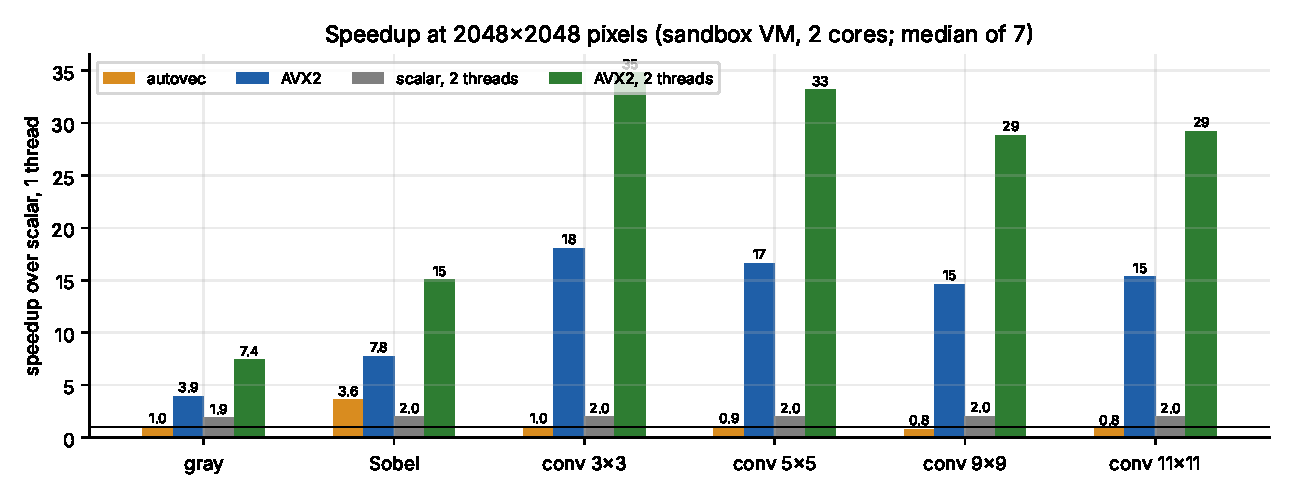
\includegraphics[width=0.95\textwidth]{figures/f_speedup.pdf}
\captionof{figure}{Speedups over single-thread scalar at 2048$\times$2048.}
\end{center}

What these data say, each point tied to a number:
\begin{itemize}
\item \textbf{AVX2 is the dominant factor.} On one thread it is \spGrayAvx$\times$ faster than scalar for gray, \spSobelAvx$\times$ for Sobel and \spConvNineAvx$\times$ (9$\times$9) to \spConvThreeAvx$\times$ (3$\times$3) for convolution; the convolution figure is lowest for the larger kernels because it is the scalar baseline that benefits from nothing and the vector kernel that approaches its FMA ceiling. The speedup of convolution is much larger than the 8 lanes of a float vector because the scalar code needs separate multiply, add, load and index instructions per tap (and cannot be auto-vectorized, see below), whereas AVX2 retires one fused multiply-add on eight pixels per instruction.
\item \textbf{GCC's auto-vectorizer helps Sobel, not gray or convolution.} It reaches \spSobelAutovec$\times$ on Sobel, but \spGrayAutovec$\times$ on gray (the vectorization report marks the loop as failed; the interleaved 3-byte RGB access is the likely cause but the report does not say so) and \spConvThreeAutovec$\times$ ($3\times3$) down to \spConvElevenAutovec$\times$ ($11\times11$) on convolution, i.e.\ no gain and for the larger kernels slightly slower than scalar (the report names the loop-nest structure, Chapter~\ref{ch:scalar}). Chapter~\ref{ch:scalar} shows the report and which of these statements the compiler makes itself and which are interpretation.
\item \textbf{OpenMP scales as the hardware allows.} With two threads scalar code gives about 2$\times$ (\spGrayScalarTwo, \spSobelScalarTwo, \spConvThreeScalarTwo), and AVX2 with two threads \spGrayAvxTwo$\times$, \spSobelAvxTwo$\times$ and \spConvThreeAvxTwo$\times$ over single-thread scalar: the two factors multiply. At 4096$\times$4096 two threads give \scaleGrayAvxFourK$\times$ (gray), \scaleSobelAvxFourK$\times$ (Sobel) and \scaleConvAvxFourK$\times$ (convolution 9$\times$9) over one thread, i.e.\ close to perfect scaling \emph{on this machine}, because two threads do not saturate its memory (Chapter~\ref{ch:cache}). That does not carry over to 32 or 64 cores: gray and Sobel will flatten once the memory system is saturated, convolution much later. The scaling script exists to measure exactly this.
\end{itemize}

\begin{center}
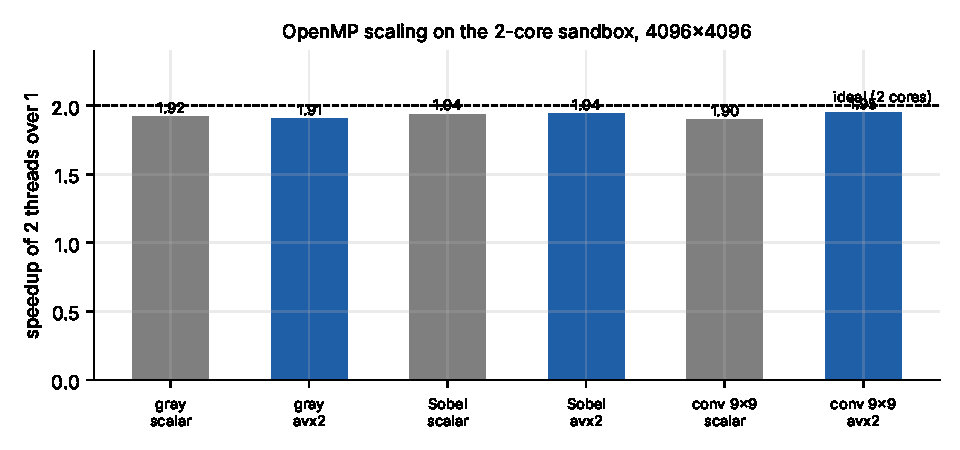
\includegraphics[width=0.8\textwidth]{figures/f_threads.pdf}
\captionof{figure}{Two threads versus one at 4096$\times$4096.}
\end{center}

\section{Convolution: kernel size and the ablations}

\begin{center}
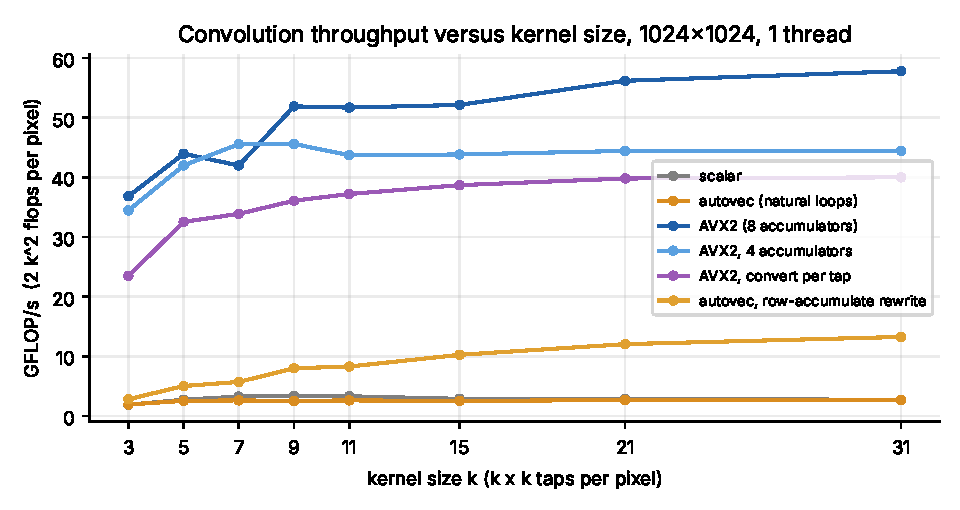
\includegraphics[width=0.85\textwidth]{figures/f_conv_ksize.pdf}
\captionof{figure}{Convolution rate versus kernel size (1024$\times$1024, one thread).}
\end{center}

\begin{center}
\small
\begin{tabular}{@{}lrrr@{}}
\toprule
GFLOP/s, 1024$^2$, 1 thread & $k=3$ & $k=9$ & $k=31$\\
\midrule
\inputrows{snippets/tab_ablation}
\end{tabular}
\end{center}

\begin{itemize}
\item \textbf{Throughput rises with $k$ and then flattens at \gfAvxMax\,GFLOP/s}, about \fracOfNominalPeak\,\% of the nominal peak of one core (Chapter~\ref{ch:cache}). For $k=3$ the fixed per-row costs (converting a row to float, writing the output) are a larger share of the work (\gfAvxThree\,GFLOP/s); for large kernels the FMA units dominate. Scalar stays below \gfScalarMax\,GFLOP/s throughout.
\item \textbf{Eight accumulators beat four}: \ratioAccFourNine$\times$ at $k=9$ and up to \ratioAccFourMax$\times$ for larger kernels: with fewer independent FMA chains the 4-cycle FMA latency is no longer hidden (Chapter~\ref{ch:conv}).
\item \textbf{Converting per tap costs} a factor \ratioPerTapNine\ at $k=9$: converting each byte to float for every tap rather than once per row spends instructions that compete with the FMAs.
\item \textbf{Helping the compiler} (the row-accumulate rewrite, bit-identical to scalar) gives \gfRowAccNine\,GFLOP/s at $k=9$, \ratioRowAccToNatural$\times$ the natural-loop autovec but still \ratioRowAccToAvx$\times$ below the hand-written kernel. The compiler got a long way once the loop was restructured; the remaining gap is plausibly the register blocking of the hand-written kernel (eight accumulators held in registers for a whole block of pixels across all $k^2$ taps); the experiment shows the gap, not its cause, and a look at the generated assembly would be needed to be sure.
\end{itemize}
Those four statements are the answer to ``why not just let the compiler do it?'': it is a measured, quantified answer.

\section{Comparison with OpenCV}

\begin{center}
\small
\begin{tabular}{@{}lrrr@{}}
\toprule
2048$\times$2048, 1 thread & OpenCV (ms) & this library, AVX2 (ms) & OpenCV / ours\\
\midrule
\inputrows{snippets/tab_opencv}
\end{tabular}
\end{center}

This comparison is useful for orientation and dangerous as a claim. The caveats are part of the result:
\begin{itemize}
\item OpenCV was installed with \code{pip} in the sandbox (version 5.0.0, 1 thread, ``optimized: True''); its build and CPU dispatch (which instruction sets it chose on this VM) were not inspected.
\item Gray: OpenCV uses 14-bit coefficients, so its output differs from ours by up to one level on 7.4\,\% of pixels: it does more precise work.
\item Sobel: our function is one fused pass producing $\min(255,|G_x|+|G_y|)$; the OpenCV figure is two \code{Sobel} calls in 16-bit, absolute values, a saturating add, i.e.\ a \emph{pipeline} of several full-image passes and temporary images. Part of the \ocvSobel$\times$ is fusion, not SIMD quality.
\item Convolution: \code{filter2D} handles border modes, depths and arbitrary kernels and allocates its output; it agrees with ours to within one level on every tested kernel (identical for $3\times3$).
\item Python call overhead is included in the OpenCV time; at 2048$^2$ it is negligible (microseconds against milliseconds).
\end{itemize}
The defensible sentence is: ``On this machine my AVX2 kernels run \ocvGray$\times$ to \ocvConvNine$\times$ faster than the corresponding OpenCV calls for gray and convolution and about \ocvSobel$\times$ for the Sobel pipeline, where most of that comes from doing it in one pass; OpenCV supports far more and I do not claim to replace it.'' The indefensible sentence is ``faster than OpenCV''.

\section{Repeatability: how big is a ``real'' difference?}

Two different spreads were measured, and the second one is the larger and the more instructive.
\begin{itemize}
\item \textbf{Within one job (E6).} The same 24 measurements repeated three times in a row differ by up to \repSpreadOne\,\% between repetitions for single-thread runs and up to \repSpreadTwo\,\% for two-thread runs (the host is shared; with two threads on a 2-vCPU guest any background activity lands on a thread of the benchmark).
\item \textbf{Between two passes minutes apart.} The main experiment (E1) was run twice with the identical command; the first pass is kept in \file{results/sandbox\_example/firstrun/}. For image sizes of 1024 and above, the median difference between the two passes was \betweenScalarMed\,\% for the scalar implementation (largest: \betweenScalarMax\,\%), \betweenAutovecMed\,\% for autovec (largest \betweenAutovecMax\,\%) and only \betweenAvxMed\,\% for AVX2 (largest \betweenAvxMax\,\%). The scalar convolution was the main culprit: in the first pass it ran slower by up to about 40\,\% on many configurations, for a reason I cannot identify from inside a virtual machine (other tenants on the host, a different clock state, or both). All numbers in this chapter come from the second pass, and the other experiments were repeated after it for consistency.
\end{itemize}
Consequences:
\begin{itemize}
\item \textbf{Speedups inherit the noise of their denominator.} The AVX2 timings are stable, the scalar baseline is not, so a speedup computed from one scalar measurement can be off by tens of percent. Quote speedups as ranges or as ``about'', and take the baseline from several runs (the minimum of several medians is a reasonable estimate of the undisturbed scalar time).
\item Differences of a few percent between two configurations, such as the stride experiment, are \emph{not} evidence.
\item Order-of-magnitude differences (the 20$\times$ of AVX2 convolution) are robust: even a 40\,\% error in the baseline does not change that conclusion.
\item On the cluster use \code{--exclusive} for the cleanest numbers, repeat the jobs at different times, and quote the minimum and the spread, not just one number. Compare partitions only with the same binary and the same sizes.
\end{itemize}

\section{What to say about performance in an interview}

\begin{sound}
``On my test machine the AVX2 kernels are about \spGrayAvx{} times faster than scalar for gray, \spSobelAvx{} for Sobel and roughly \spConvNineAvx{} to \spConvThreeAvx{} for convolution, and OpenMP multiplies that by the core count until memory bandwidth takes over. I also measured four design decisions on the convolution: eight accumulators versus four, converting once per row instead of per tap, hand-written versus a compiler-friendly rewrite, and I can show you why each matters. The AVX2 timings repeated within a couple of percent, the scalar baseline moved by tens of percent between two passes, so I quote speedups as approximate and only draw conclusions from large differences. The cluster numbers I measured with the same scripts on bwUniCluster are \dots''
\end{sound}
(Fill the last sentence from your own cluster runs, and only from them.)

\chapter{Running it yourself: build, tools, experiments}\label{ch:running}

Everything in this chapter works on any Linux machine with GCC (C++17, OpenMP) and an x86-64 CPU with AVX2 and FMA; the Python scripts need Python 3 with NumPy and SciPy (OpenCV is optional). On a CPU without AVX2 the library still builds; the AVX2 paths report ``not supported'' and the tests skip them.

\section{Project layout}

\begin{center}
\small
\begin{tabularx}{\textwidth}{@{}lX@{}}
\toprule
\file{include/simdip/} & the public API: \file{image.hpp}, \file{kernel.hpp}, \file{ops.hpp}\\
\file{src/} & \file{scalar\_impl.inc} (the one scalar source, included twice), \file{scalar\_novec.cpp}, \file{scalar\_autovec.cpp}, \file{avx2.cpp}, \file{dispatch.cpp} (validation, OpenMP bands, impl choice), \file{reference.cpp}, \file{image.cpp}, \file{kernel.cpp}\\
\file{apps/} & \file{simdip\_cli.cpp} (command line tool), \file{simdip\_bench.cpp} (benchmark harness)\\
\file{tests/} & \file{test\_main.cpp}: 24 test groups, no framework needed\\
\file{python/} & independent NumPy reference, cross-check, OpenCV comparison, experiment runner, figure generator\\
\file{scripts/} & \file{mutation\_test.sh}\\
\file{slurm/} & job scripts for bwUniCluster\\
\file{results/} & saved sandbox example results, logs of tests, cross-check and mutation runs\\
\file{docs/} & the \LaTeX\ sources of this guide\\
\bottomrule
\end{tabularx}
\end{center}

\section{Build and test}

\begin{lstlisting}[style=shell]
make -j4                  # library, CLI, benchmark, tests -> build/
make test                 # 24 groups; the last line must read "... 0 failures"
make asan-test            # same tests with AddressSanitizer + UBSan (build_asan/)
make vec-report           # what GCC auto-vectorized -> build/vec_report_full.txt
make OPT="-O3 -march=native" BUILD=build_native    # let the compiler use the whole CPU (autovec only)
make OPENMP=0             # no OpenMP; the threads argument is ignored
\end{lstlisting}

The per-file compiler flags are in the Makefile and are part of the design (Chapter~\ref{ch:scalar}): \code{scalar\_novec.cpp} with the vectorizer off, \code{scalar\_autovec.cpp} with it on, both with \code{-ffp-contract=off}, and \code{avx2.cpp} with \code{-mavx2 -mfma}. A program that links the library calls AVX2 code only after the run-time CPU check \code{avx2Supported()}.

\section{The command-line tool}

\begin{lstlisting}[style=shell]
./build/simdip info                                   # CPU features, threads
python3 python/make_test_images.py                    # writes data/*.pgm, data/*.ppm
./build/simdip gray  data/astronaut.ppm  out_gray.pgm --impl avx2 --threads 2
./build/simdip sobel data/camera.pgm     out_sobel.pgm --impl avx2
./build/simdip conv  data/camera.pgm     out_blur.pgm --kernel gauss --size 9 --sigma 2.5 --impl avx2
./build/simdip conv  data/camera.pgm     out_sharp.pgm --kernel sharpen --impl scalar
\end{lstlisting}
Images are read and written as PNM (PGM for gray, PPM for colour). View them with any image viewer that supports PNM, or convert them with OpenCV or Pillow (for example \code{cv2.imwrite} on the result of \code{cv2.imread}). Running the same command with \code{--impl scalar} and \code{--impl avx2} and comparing the files with \code{cmp} is the quickest sanity check: for gray and Sobel they must be identical.

\section{The benchmark tool}

\begin{lstlisting}[style=shell]
./build/simdip_bench --op gray,sobel,conv --impl scalar,autovec,avx2 \
    --sizes 512,1024,2048 --ksizes 3,5,9 --threads 1,2 --reps 9 --csv out.csv --label try1
./build/simdip_bench --op conv --impl avx2 --ablation --sizes 1024 --ksizes 3,9,31 --csv abl.csv
./build/simdip_bench --op copy --sizes 4096 --threads 1,2       # memory-bandwidth yardstick
./build/simdip_bench --op sobel,conv --sizes 4096 --stride 4160 --ksizes 9   # explicit row stride
\end{lstlisting}
Options: \code{--op} (gray, sobel, conv, copy), \code{--impl}, \code{--sizes} (image side in pixels), \code{--ksizes}, \code{--threads}, \code{--reps}, \code{--min-ms}, \code{--stride} (bytes), \code{--aspect N} (height $=$ width$/N$, for non-square images), \code{--ablation}, \code{--csv}, \code{--label}. The CSV has one row per measurement with the columns \code{label, op, impl, threads, width, height, stride, ksize, iters, reps, median\_ms, min\_ms, max\_ms, mpix\_s, gb\_s, gflops}. Build with \code{-O0} and the program prints a warning that the timings are meaningless.

\section{Python scripts}

\begin{center}
\small
\begin{tabularx}{\textwidth}{@{}lX@{}}
\toprule
\file{make\_test\_images.py} & generates the test pictures (a photograph, colour images, noise, a checkerboard) into \file{data/}\\
\file{ref\_numpy.py} & the independent reference implementation (NumPy + SciPy)\\
\file{crosscheck.py} & runs the CLI for all implementations and thread counts, compares with the reference; prints the number of comparisons and mismatches\\
\file{compare\_opencv.py} & agreement and speed comparison against OpenCV (needs \code{cv2}); \code{--bench-csv}, \code{--size}, \code{--out}\\
\file{run\_experiments.py} & reruns the experiments E1--E5 into \file{results/}\\
\file{make\_figures.py} & produces every figure, table and number macro used in this PDF from the CSV files\\
\file{extract\_code.py} & cuts the code listings of this guide out of the source files (so listings cannot drift from the code)\\
\bottomrule
\end{tabularx}
\end{center}

\section{Experiments}

\begin{center}
\small
\begin{tabularx}{\textwidth}{@{}llX@{}}
\toprule
id & file & question\\
\midrule
E1 & \file{E1\_main.csv} & every op $\times$ implementation $\times$ size $\times$ kernel, 1 and 2 threads\\
E2 & \file{E2\_sizes.csv} & throughput versus image size (cache effects)\\
E3 & \file{E3\_stride\_*.csv} & row stride equal to a page multiple versus padded by 64 bytes\\
E4 & \file{E4\_ksize.csv} & convolution versus kernel size, with the three ablations\\
E5 & \file{E5\_copy.csv} & the memory-bandwidth yardstick (\code{memcpy})\\
E6 & \file{E6\_repeat\_*.csv} & the same measurement three times: repeatability\\
E7 & \file{E7\_scaling.csv} & (cluster) OpenMP scaling 1 to 32 threads; not available in the sandbox (2 cores)\\
\bottomrule
\end{tabularx}
\end{center}

\section{Using the library from your own code}

\begin{lstlisting}
#include "simdip/ops.hpp"
using namespace simdip;

Image rgb = readPNM("in.ppm");                    // 3 channels
Image gray(rgb.width(), rgb.height(), 1);         // destination: right size, 1 channel
rgbToGray(rgb, gray, {Impl::Avx2, 4});            // AVX2, 4 OpenMP threads
Image edges(gray.width(), gray.height(), 1);
sobel(gray, edges, {Impl::Avx2, 4});
Image blurred(gray.width(), gray.height(), 1);
convolve(gray, blurred, kernels::gaussian(9, 2.5), {Impl::Avx2, 4});
\end{lstlisting}
The functions throw \code{std::invalid\_argument} for wrong sizes, overlapping buffers or an unusable kernel; they never read or write outside the pixels of a row.

\chapter{Running on bwUniCluster 3.0: step by step}\label{ch:cluster}

bwUniCluster 3.0 is the shared HPC system operated by KIT for universities in Baden-W\"urttemberg, including Freiburg. You use it by logging in to a \emph{login node}, preparing your work there, and handing the real computation to a job scheduler called \textbf{Slurm}, which runs it on a \emph{compute node}.

\begin{plain}
\textbf{Mental model.} The login node is a shared reception desk: fine for editing files and submitting forms, \emph{not} for computing (heavy computations on login nodes are not allowed). The compute nodes are the workshops. A \emph{job script} is the form you hand in: ``give me 1 core for 30 minutes on an Intel node, then run these commands''. Slurm queues the form and runs it when a node is free.
\end{plain}

\begin{warn}[Facts and where they come from]
Queue names, limits and hardware below come from the official bwHPC wiki pages listed at the end of this chapter, which I read while preparing this guide. HPC sites change these things. Before relying on a number, confirm it on the cluster with \code{sinfo -s} (queues), \code{module avail} (software) and the wiki.
\end{warn}

\section{The workflow in one picture}

\begin{center}
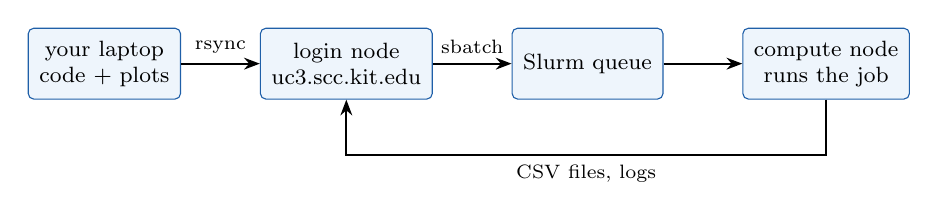
\begin{tikzpicture}[node distance=0.5cm,
  b/.style={draw=accent,fill=plainbg,rounded corners=2pt,minimum height=0.9cm,align=center,font=\footnotesize,inner sep=4pt},
  arr/.style={-{Stealth[length=2mm]},thick}]
\node[b] (a) {your laptop\\code + plots};
\node[b,right=1cm of a] (b) {login node\\\texttt{uc3.scc.kit.edu}};
\node[b,right=1cm of b] (c) {Slurm queue};
\node[b,right=1cm of c] (d) {compute node\\runs the job};
\draw[arr] (a) -- node[above,font=\scriptsize]{rsync} (b);
\draw[arr] (b) -- node[above,font=\scriptsize]{sbatch} (c);
\draw[arr] (c) -- (d);
\draw[arr] (d.south) -- ++(0,-0.7) -| node[pos=0.25,below,font=\scriptsize]{CSV files, logs} (b.south);
\end{tikzpicture}
\end{center}

\section{One-time setup: account and login}

\begin{enumerate}
\item \textbf{Registration.} The login documentation lists three prerequisites: complete the 3-step registration procedure, set a \emph{service password} for bwUniCluster 3.0, and set up a \emph{second factor} (a TOTP app on your phone). You enter the one-time code first and then the service password when you log in. If you have used the cluster before, this is probably done; if the login fails, this is the first thing to re-check.
\item \textbf{Network.} Access is limited to the BelW\"u research network. On the Freiburg campus network you are normally inside it; from home use the university VPN or an SSH jump host. A connection that times out from outside is not a bug in your command.
\item \textbf{Log in.}
\begin{lstlisting}[style=shell]
ssh <your_username>@uc3.scc.kit.edu
\end{lstlisting}
Your username is a university prefix plus your local name (for KIT users, for example, \code{ka\_ab1234}); the registration pages show yours. Alternative host names listed on the wiki: \code{bwunicluster.scc.kit.edu}, \code{uc3-login1.scc.kit.edu}, \code{uc3-login2.scc.kit.edu}.
\end{enumerate}

\section{Where to put files}

\begin{center}
\small
\begin{tabular}{@{}p{3.1cm}p{11.5cm}@{}}
\toprule
\code{\$HOME} & Permanent, backed up, same on all nodes. Put source code and job scripts here. Our project is a few megabytes, so it lives here.\\
\textbf{Workspaces} & For large temporary data (restart files, big outputs). Created with \code{ws\_allocate <name> <days>}, found with \code{ws\_find <name>}, listed with \code{ws\_list}, extended with \code{ws\_extend <name> <days>}; they expire. You do not need one for this project unless you benchmark with many gigabytes of images.\\
\code{\$TMPDIR} & Fast node-local disk, exists only while a job runs. Irrelevant here.\\ \bottomrule
\end{tabular}
\end{center}

\section{Step 1: copy the project to the cluster}

From your laptop (in the folder that contains \code{simd\_imgproc/}):
\begin{lstlisting}[style=shell]
rsync -av --exclude 'build*' --exclude results/sandbox_example simd_imgproc/ <user>@uc3.scc.kit.edu:~/simd_imgproc/
\end{lstlisting}
(Or push to a private GitHub repository and \code{git clone} on the cluster.) Then on the cluster:
\begin{lstlisting}[style=shell]
cd ~/simd_imgproc
mkdir -p logs results data
\end{lstlisting}
The C++ benchmark uses synthetic images and needs no data files. The cross-check needs the test images; \code{data/} is included in the package already, so the rsync above copies it.

\section{Step 2: look around}

\begin{lstlisting}[style=shell]
module avail compiler/gnu        # which GNU compiler versions exist
module spider gnu                # (Lmod) also finds modules with unmet dependencies
sinfo -s                         # summary of queues (partitions) and node counts
squeue --me                      # your own jobs
lscpu | grep -E 'Model name|Flags' | head   # does the node you land on list avx2 and fma?
\end{lstlisting}
The cluster uses \textbf{Lmod}: \code{module load}, \code{module list}, \code{module purge} and \code{module spider} are the commands you need. The wiki lists GNU compilers \code{compiler/gnu/11.4} and \code{compiler/gnu/14.2} (\code{13.3} is also referenced). \file{slurm/env.sh} tries \code{compiler/gnu/14.2} first and falls back to the default \code{compiler/gnu}; edit it if \code{module avail} shows different versions. The project needs C++17 and OpenMP. It was built and tested with GCC 13.3; any recent GCC should work, but older ones were not tried.

\section{The queues you will use}

\begin{center}
\small
{\small\setlength{\tabcolsep}{4pt}\begin{tabular}{@{}lllll@{}}
\toprule
\textbf{queue} & \textbf{node type} & \textbf{cores / memory} & \textbf{max wall time} & \textbf{use it for}\\ \midrule
\code{dev\_cpu} & development queue & as \code{cpu} & 30 min & compile, test, short checks\\
\code{cpu\_il} & Intel Xeon Platinum 8358 (Ice Lake) & 64 cores, 256\,GiB & 72 h & benchmark\\
\code{cpu} & AMD EPYC 9454 & 96 cores, 384\,GiB & 72 h & benchmark\\
\code{highmem} & AMD EPYC 9454 & 96 cores, 2.3\,TiB & 72 h & not needed\\
\bottomrule
\end{tabular}}
\end{center}

\textbf{Development queues} (\code{dev\_} prefix) have a 30-minute limit, allow only \emph{one running job at a time} and at most 3 queued, and are meant for ``developing, compiling and testing code''. The wiki says not to misuse them for regular short-running production jobs. So: build and test in \code{dev\_cpu}; run the benchmarks in \code{cpu\_il} and \code{cpu}.

\begin{warn}[Both CPUs have AVX2 and FMA; the sandbox numbers do not transfer]
The library's AVX2 path needs AVX2 and FMA; the two benchmark partitions use CPUs of generations that provide both, but confirm it on the node with \code{lscpu} (the job's \file{meta.txt} records the CPU model). The two partitions differ in core count, caches, memory bandwidth and clock, so you will get \emph{two different tables}, and both differ from the sandbox. That is the point of running both.
\end{warn}

\section{Step 3: build and test on a compute node}

\begin{lstlisting}[style=shell]
sbatch slurm/01_build_test.sbatch
squeue --me                       # PD = pending, R = running. Check again after a minute or two.
cat logs/simdip-build_<jobid>.out # expect "... 0 failures" twice (normal build and sanitizer build) and "build + tests OK"
\end{lstlisting}

\begin{warn}[Be kind to the scheduler]
The wiki asks you not to run \code{squeue} or other Slurm commands in loops or with \code{watch}, and to leave at least 30 seconds between queries. Submit, wait, check.
\end{warn}

The job runs the unit tests, then the AddressSanitizer build of the same tests, then the NumPy cross-check if \code{python3} has NumPy and SciPy (otherwise it prints a message and skips it, which is not a failure). The test log is saved as \file{results/test\_log\_cluster.txt}. Interactive alternative (from the wiki):
\begin{lstlisting}[style=shell]
salloc -p dev_cpu -n 1 -t 20 --mem=4000      # 1 task, 20 minutes, 4000 MB; you land on the node
module load compiler/gnu && make && make test
exit                                          # give the node back!
\end{lstlisting}

\section{Step 4: the benchmark jobs}

\begin{lstlisting}[style=shell]
bash slurm/submit_all.sh          # 2 jobs per partition: single-core (02) and OpenMP scaling (03)
squeue --me
\end{lstlisting}

\begin{center}
\small
\begin{tabularx}{\textwidth}{@{}llX@{}}
\toprule
script & resources & what it measures\\
\midrule
\file{02\_bench\_single.sbatch} & 2 cores, 12\,GB, 1.5 h & the same experiment set as the sandbox example: E1 (all ops, implementations, sizes 256--4096, kernels 3--11, 1 and 2 threads), E2 (size sweep), E3 (page-multiple stride versus +64 B), E4 (kernel sizes up to 31 with ablations), E5 (\code{memcpy} yardstick), E6 (repeatability), plus the OpenCV comparison if \code{cv2} is available. Results in \file{results/<partition>/}.\\
\file{03\_bench\_scaling.sbatch} & 32 cores, 24\,GB, 1 h & E7: threads 1, 2, 4, 8, 16, 32 for scalar and AVX2, sizes 2048, 4096, 8192; also the \code{memcpy} yardstick with the same thread counts. Threads pinned with \code{OMP\_PROC\_BIND=close}, \code{OMP\_PLACES=cores}.\\
\file{04\_profile.sbatch} & 2 cores, \code{dev\_cpu} & compiler vectorization report and a gprof flat profile of the scalar and autovec code\\
\bottomrule
\end{tabularx}
\end{center}

\subsection{What the \#SBATCH lines mean}

\begin{center}
\small
\begin{tabular}{@{}p{4.6cm}p{10cm}@{}}
\toprule
\code{--partition=cpu\_il} & Which queue (node type). Overridden by \code{sbatch --partition=cpu ...}.\\
\code{--nodes=1 --ntasks=1} & One node, one process.\\
\code{--cpus-per-task=1} (or 32) & How many cores the process may use. The benchmark job asks for two cores because it also times 2 threads; its single-thread numbers use one of them; the scaling job asks for 32 and sets \code{OMP\_NUM\_THREADS} from it.\\
\code{--mem=12000mb} & Memory. The largest image here (8192$^2$) needs well under 1\,GB; ask explicitly because the default per core is small.\\
\code{--time=01:00:00} & Wall-time limit. The job is killed at the limit.\\
\code{--output=logs/\%x\_\%j.out} & Log file: \code{\%x} = job name, \code{\%j} = job number. \textbf{The directory must already exist} (\code{mkdir -p logs}) or the job fails immediately.\\
\code{srun --cpu-bind=cores} & Starts the program on the allocated core and pins it so it cannot migrate during the measurement. The scaling job uses \code{--cpu-bind=none} and lets OpenMP do the pinning.\\ \bottomrule
\end{tabular}
\end{center}

\subsection{Benchmark hygiene (what makes a number trustworthy)}

\begin{itemize}
\item \textbf{Warm-up, repetitions, median} are built into \code{simdip\_bench}; the spread is in the CSV (\code{min\_ms}, \code{max\_ms}).
\item \textbf{Same binary, same input, same settings} on both partitions; only the node changes.
\item \textbf{The node may be shared.} Other jobs on the same node disturb timings, in particular memory bandwidth, which is what the multi-thread results measure. For the scaling job the clean version is \code{sbatch --exclusive --partition=cpu\_il slurm/03\_bench\_scaling.sbatch} (longer queue wait). A scaling curve measured on a busy node says more about the neighbours than about your code.
\item \textbf{Repeat.} Run each job at least twice at different times and compare. The E6 block inside the job measures the spread within one job; the spread \emph{between} jobs can be larger (in the sandbox the scalar baseline differed by a median of \betweenScalarMed\,\% and up to \betweenScalarMax\,\% between two passes of the same command, Chapter~\ref{ch:bench}).
\item \textbf{Report what you measured}: ``median of 9 samples, single core, GCC \dots, \code{-O3}, partition \dots, node \dots''.
\item \textbf{Optional extra:} \code{NATIVE=1 sbatch --partition=cpu\_il slurm/02\_bench\_single.sbatch} rebuilds with \code{-march=native} on the compute node into a separate build directory and results folder \file{results/<partition>\_native/}. The ``autovec'' column may then use AVX2 or AVX-512 and FMA contraction is still off for that file. Compare with the portable build. A native binary can fail with ``illegal instruction'' on a different CPU type, so it is named per partition.
\end{itemize}

\section{Step 5: profile}

\begin{lstlisting}[style=shell]
sbatch slurm/04_profile.sbatch       # dev_cpu, about 2 minutes
less results/vec_report_cluster.txt  # which loops did this GCC vectorize?
less results/gprof_flat.txt          # function-level table
\end{lstlisting}
The vectorization report is the cluster compiler's answer to Chapter~\ref{ch:scalar}: a newer or older GCC can make different decisions, and that is a legitimate thing to report.

\section{Step 6: bring the results home}

\begin{lstlisting}[style=shell]
rsync -av <user>@uc3.scc.kit.edu:~/simd_imgproc/results/ ./cluster_results/
\end{lstlisting}
Then turn them into the same figures and tables as in this guide, without touching the guide's own files:
\begin{lstlisting}[style=shell]
python3 python/make_figures.py --results cluster_results/cpu_il --out cluster_results/cpu_il/report \
        --testlog cluster_results/test_log_cluster.txt --crosslog cluster_results/crosscheck_log_cluster.txt
\end{lstlisting}
This writes \file{report/figures/*.pdf} (speedups, size sweep, kernel sizes, bandwidth, stride, and \file{f\_scaling.pdf} from the scaling job) and \file{report/snippets/*.tex} (tables and number macros). It needs Python with NumPy, SciPy and matplotlib on your laptop; the \code{--testlog}/\code{--crosslog} options can be left out if you only want the benchmark tables. Where the guide's text quotes a sandbox number, read your own value in the corresponding table instead; the chapters were written around the structure of the results, not around a specific machine.

\section{When something goes wrong}

\begin{center}
\small
\begin{tabular}{@{}p{4.4cm}p{10.2cm}@{}}
\toprule
\textbf{Symptom} & \textbf{Likely cause and fix}\\ \midrule
\code{ssh} hangs or is refused & Not in the BelW\"u network: connect to the university VPN. Wrong code order: one-time code first, then service password.\\
\code{module: command not found} in a script & The script is not run through a login shell. \file{slurm/env.sh} checks for it; check \code{module list} at the top of the log.\\
Module not found & Version differs: \code{module avail compiler/gnu}, \code{module spider gnu}, then edit \file{slurm/env.sh}.\\
Job stays \code{PD} (pending) & Normal. \code{squeue --me} shows a reason: \code{Priority}/\code{Resources} = waiting for a free node; for \code{dev\_cpu} you may only have one running job.\\
Job fails in 1 second, empty log & \code{logs/} directory missing, or a typo in \code{--partition}. Look at \code{scontrol show job <id>} and run \code{sinfo -s}.\\
\code{Killed} / out-of-memory & Raise \code{--mem}.\\
Benchmark prints ``avx2+fma: no'' & The node's CPU lacks AVX2/FMA or the job landed somewhere unexpected; check \file{meta.txt}. AVX2 rows are skipped automatically.\\
``Illegal instruction'' & A \code{-march=native} binary ran on a different CPU type; rebuild on the node that runs it.\\
Scaling curve flat after a few threads & Expected for gray and Sobel when memory bandwidth saturates; check against the \code{memcpy} scaling in \file{E7\_copy\_scaling.csv}. Also check the \code{OMP\_PROC\_BIND} line printed at the top of the output.\\
Numbers differ a lot between runs & Shared node. Use \code{--exclusive}, more repetitions, or compare medians from separate runs.\\
Tests fail on the cluster but not locally & Should not happen; the results are deterministic. Check \code{g++ --version} and that the sources are current, then investigate: it would be a real finding.\\ \bottomrule
\end{tabular}
\end{center}

\section{How to describe it truthfully}

After you have run the jobs, a sentence you can use, with the brackets filled from \emph{your} CSV files:
\begin{quote}
``I benchmarked the library on bwUniCluster 3.0 nodes (Intel Xeon Platinum 8358 and AMD EPYC 9454) with GCC and \code{-O3}: single core, median of 9 samples, AVX2 versus scalar speedups of [\dots] for gray, [\dots] for Sobel and [\dots] for 5$\times$5 convolution, and OpenMP scaling to [\dots] threads, where gray and Sobel flattened at [\dots] threads because of memory bandwidth.''
\end{quote}
Only claim what the logs and \file{meta.txt} show. If something did not run, say so. If you have older cluster numbers from a previous version of this project, do not mix them with these.

\section{Sources}

All retrieved while preparing the project-2 guide and reused here unchanged; re-check them, since clusters change.
\begin{itemize}\small
\item Batch queues: \url{https://wiki.bwhpc.de/e/BwUniCluster3.0/Batch_Queues}
\item Running jobs (\code{sbatch}, \code{salloc}, monitoring): \url{https://wiki.bwhpc.de/e/BwUniCluster3.0/Running_Jobs}
\item Software modules (Lmod): \url{https://wiki.bwhpc.de/e/BwUniCluster3.0/Software_Modules}
\item Login, registration, network restriction: \url{https://wiki.bwhpc.de/e/BwUniCluster3.0/Login}
\item Hardware and file systems: {\small\url{https://wiki.bwhpc.de/e/BwUniCluster3.0/Hardware_and_Architecture}}
\item Workspaces: \url{https://wiki.bwhpc.de/e/Workspaces}
\end{itemize}

\chapter{The resume bullets, one by one}\label{ch:resume}

\begin{warn}[Wording]
The bullets below are paraphrased from the project description (``optimized grayscale conversion, Sobel edge detection and 2D convolution; scalar, OpenMP and AVX2 implementations; vectorized operations and cache-aware memory access; benchmarks of runtime, throughput and speedup across resolutions and kernel sizes; automated correctness tests against a scalar reference''). Replace the quoted lines with your exact resume text; the explanations stay valid. Anything in square brackets is a number you must take from your own cluster runs.
\end{warn}

For each bullet: what it means in plain words, how it was done, where to find it, what evidence exists, and the follow-up question to expect.

\section{Bullet 1: three operations, three implementations}
\textit{``Implemented grayscale conversion, Sobel edge detection and 2D convolution in C++ with scalar, OpenMP-parallel and AVX2-vectorized versions.''}

\begin{description}[leftmargin=2.2cm,style=nextline]
\item[What] Three image operations, each in three implementation styles (scalar, compiler-vectorized, hand-written AVX2), each runnable on 1 to $n$ OpenMP threads: $3\times3\times$ threads, all producing the same pixels.
\item[How] One scalar source compiled two ways; AVX2 intrinsics in one translation unit with run-time CPU check; row-band parallelism with \code{omp parallel} over contiguous bands (Chapters~\ref{ch:scalar}--\ref{ch:conv}).
\item[Where] \file{src/scalar\_impl.inc}, \file{src/avx2.cpp}, \file{src/dispatch.cpp}.
\item[Evidence] \testGroups\ test groups; AVX2 results equal an independent \code{fmaf} reference bit for bit; gray verified on all $2^{24}$ colours.
\item[Expect] ``Walk me through the AVX2 grayscale.'' (3 loads of 16 bytes, 9 \code{pshufb} to deinterleave R, G, B, widen to 16 bits, multiply by 77/150/29, add 128, shift right 8, pack; Chapter~\ref{ch:gray}.) ``Why not float for gray?'' (Integer keeps 16 pixels per register and exactness; 8-bit coefficients cost 0.2\,\% coefficient error.)
\end{description}

\section{Bullet 2: vectorization and cache-aware access}
\textit{``Optimized for cache and SIMD: vectorized arithmetic, aligned rows, a ring of converted rows for convolution, register blocking with independent accumulators.''}

\begin{description}[leftmargin=2.2cm,style=nextline]
\item[What] The arithmetic is data-parallel across pixels, and the data re-used by neighbouring outputs is kept in cache or registers.
\item[How] 64-byte-aligned rows; stride that avoids exact multiples of 4096 bytes; convolution converts each source row to float \emph{once} into a ring of $k$ padded rows (the working set is $4k(w+2r)$ bytes, in L2); eight independent accumulators to hide FMA latency; one broadcast weight per tap.
\item[Where] \code{convolveRowsImpl$<$8$>$} in \file{src/avx2.cpp}; Chapters~\ref{ch:conv} and~\ref{ch:cache}.
\item[Evidence] Ablations on the convolution (Chapter~\ref{ch:bench}): 8 accumulators are \ratioAccFourNine$\times$ faster than 4 at $k=9$; converting per tap costs \ratioPerTapNine$\times$; the compiler-friendly rewrite reaches only about 1/\ratioRowAccToAvx\ of the hand-written kernel's rate. Stride experiment: effect within noise on the sandbox.
\item[Expect] ``Does the stride padding actually help?'' (Say what you measured: on the VM, within noise; the theoretical failure mode is real, and you repeat the test on the cluster.) ``How close to peak?'' (About \fracOfNominalPeak\,\% of the nominal FMA peak on the sandbox core; give your cluster figure.)
\end{description}

\section{Bullet 3: benchmarking across resolutions and kernel sizes}
\textit{``Benchmarked runtime, throughput and speedup across image resolutions and kernel sizes.''}

\begin{description}[leftmargin=2.2cm,style=nextline]
\item[What] A harness with warm-up, calibrated iteration counts, median of repetitions, CSV output, and a memory-bandwidth yardstick.
\item[How] \file{apps/simdip\_bench.cpp}; experiments E1--E7 (Chapter~\ref{ch:running}); Slurm jobs for two CPU types; figures from \file{python/make\_figures.py}.
\item[Where] Chapters~\ref{ch:bench} and~\ref{ch:cluster}.
\item[Key numbers to prepare (yours)] AVX2 over scalar, single core: gray [\,\,], Sobel [\,\,], convolution $3\times3$ [\,\,] and $9\times9$ [\,\,], on \code{cpu\_il} and on \code{cpu}; OpenMP scaling to [\,\,] threads and the thread count at which gray and Sobel stop scaling; memcpy bandwidth.
\item[Expect] ``Why does gray stop scaling before convolution does?'' (Memory bound versus compute bound; show the roofline argument and the memcpy scaling curve.) ``How reproducible are your numbers?'' (State the spread you measured, Chapter~\ref{ch:bench}.)
\end{description}

\section{Bullet 4: correctness testing}
\textit{``Developed automated correctness tests comparing all implementations against a scalar reference.''}

\begin{description}[leftmargin=2.2cm,style=nextline]
\item[What] A layered test suite whose job is to catch the bugs specific to SIMD code.
\item[How] Edge-size matrix around vector widths, padded and unpadded images, 1 to 200 threads, bit-exact comparisons, exhaustive gray, property tests, AddressSanitizer, an independent NumPy/SciPy cross-check, and a mutation test of the suite itself (\mutKilled\ of \mutTotal\ seeded bugs caught; Chapter~\ref{ch:testing}).
\item[Evidence] \testChecks\ checks, \testFailures\ failures; \crossComparisons\ cross-check comparisons, \crossMismatches\ mismatches.
\item[Expect] ``What bug did the tests find?'' (The over-read in the vector loop that the scalar tail masked; found by the mutation test because the allocator hid it.) ``How do you test floating-point code?'' (Fixed accumulation order, an FMA reference for bit-exactness, exact kernels for zero tolerance, a proven error bound for the rest.)
\end{description}

\section{Bullet 5: Python tooling}
\textit{``Python for reference implementation, cross-validation, experiment automation and plotting.''}

\begin{description}[leftmargin=2.2cm,style=nextline]
\item[What] An independent implementation of the specification, tools that drive the C++ binaries, and the figure generator.
\item[Where] \file{python/ref\_numpy.py}, \file{crosscheck.py}, \file{compare\_opencv.py}, \file{run\_experiments.py}, \file{make\_figures.py}.
\item[Expect] ``Why a second implementation in Python?'' (It shares no code and no misunderstanding with the C++ reference; it catches specification errors that self-consistency cannot.)
\end{description}

\section{Wording to consider once your cluster numbers exist}

Candidate bullets that survive a skeptical read, each fact checkable in the project:
\begin{itemize}
\item \textit{Built a C++17 image-processing library (RGB-to-gray, Sobel, $k\times k$ convolution) with scalar, auto-vectorized and hand-written AVX2 paths plus OpenMP row-band parallelism; AVX2 output is bit-identical to an independent FMA reference and gray is verified on all $2^{24}$ inputs.}
\item \textit{Designed an AVX2 convolution around a ring of float-converted rows (L2-resident), eight independent FMA accumulators and run-time CPU dispatch; reached [X]\,\% of single-core FMA peak and [Y]$\times$ over scalar on bwUniCluster (Xeon 8358), [Z]$\times$ on EPYC 9454.}
\item \textit{Quantified optimization choices with ablations (accumulator count, convert-once, compiler rewrite) and a roofline analysis using a measured memcpy yardstick; gray/Sobel saturate memory bandwidth at [N] threads, convolution scales to [M].}
\item \textit{Verified with \testChecks{} checks, AddressSanitizer, a NumPy/SciPy cross-check and mutation testing (\mutKilled/\mutTotal{} seeded bugs detected).}
\end{itemize}
Remove any bracketed claim you did not measure. Do not write ``faster than OpenCV'' (Chapter~\ref{ch:bench}), do not write a speedup that is not from your cluster run, and do not write ``cache-optimized'' unless you can describe, in one sentence, what is in which cache.

\chapter{Interview questions and answers}\label{ch:qa}

\newcommand{\qa}[2]{\par\medskip\noindent\textbf{Q. #1}\par\noindent #2\par}

Answers are written to be said aloud in 20--60 seconds. Numbers that depend on the machine are marked \emph{[yours]}: use your cluster value, or say ``on my test machine'' if you quote the sandbox figure.

\section{Orientation}

\qa{Describe the project in thirty seconds.}{A C++ image-processing library with three operations, RGB-to-gray, Sobel edge strength and $k\times k$ convolution, each in a scalar version, a compiler-vectorized version and a hand-written AVX2 version, and each parallelizable over rows with OpenMP. I wrote a test suite that checks all combinations against a reference, including bit-exact checks for the floating-point convolution, and a benchmark harness whose results I measured on bwUniCluster. The point was to understand what the hardware does with these kernels and to be able to explain each speedup.}

\qa{What is the single most important result?}{That the three kernels sit at different places on the roofline. Gray and Sobel stream pixels and end up limited by memory bandwidth after vectorization; convolution does $2k^2$ flops per pixel and is limited by the FMA units. So the extra work of intrinsics paid off most for convolution \emph{[yours: AVX2 over scalar single core]}, and OpenMP scaling flattens for gray and Sobel when bandwidth saturates \emph{[yours: thread count]}.}

\qa{What would you do differently or next?}{Row blocking in the convolution (compute two or four output rows from each loaded float row to cut loads), separable-kernel detection (a $k\times k$ separable kernel is $2k$ taps instead of $k^2$), non-temporal stores for large images, an AVX-512 path with a run-time dispatch, first-touch parallel initialisation for NUMA, and a GPU port of the same three kernels for comparison.}

\section{SIMD and AVX2}

\qa{What is SIMD, and what is the vector width here?}{One instruction operating on several data elements. An AVX2 register is 256 bits: 32 bytes, 16 16-bit integers or 8 floats. Gray and Sobel process 16 pixels per iteration in 16-bit lanes; the convolution processes 8 pixels per FMA, 64 per block of 8 accumulators.}

\qa{Why 16-bit lanes for gray and Sobel?}{The intermediate values fit: the gray sum is at most 65\,408 (unsigned 16-bit); Sobel magnitudes at most 2040 (signed 16-bit). Using 32-bit lanes would halve the pixels per instruction for no benefit.}

\qa{AVX2 \code{packus} gives scrambled pixel order. Why, and how do you fix it?}{AVX2 integer instructions mostly work independently in each 128-bit half. \code{packus} packs the low halves of both inputs into the low half of the result and the high halves into the high half, so the 64-bit quarters come out in the order 0, 2, 1, 3. A \code{permute4x64} with the right selector (or \code{permutevar8x32} after a 32-bit pack) restores the order.}

\qa{How do you deinterleave RGB in the grayscale kernel?}{Three 16-byte loads cover 16 pixels (48 bytes). Each of R, G, B is spread over all three registers in a stride-3 pattern, so for each colour I use one \code{pshufb} per register with a constant mask that picks the right bytes (and zeros the others with index \code{0x80}), then OR the three results. 9 shuffles and 6 ORs. The masks are compile-time constants.}

\qa{Why do the loads happen at \code{x-1}, \code{x} and \code{x+1} in Sobel rather than shuffling?}{Unaligned loads on current cores are cheap when they do not cross a cache line, and three loads per row avoids lane-crossing shuffles. The price is some redundant cache traffic, which stays in L1.}

\qa{Aligned versus unaligned loads: does it matter?}{On recent Intel and AMD cores an unaligned load that stays within a cache line costs the same as an aligned one; one that splits a line costs more. I align the rows to 64 bytes so that row starts are line-aligned, but kernels read at arbitrary $x$, so I use unaligned instructions throughout.}

\qa{What happens on a CPU without AVX2?}{The library checks \code{\_\_builtin\_cpu\_supports} at run time and throws if AVX2 is requested but not available; scalar and autovec still work. The AVX2 file is the only one compiled with \code{-mavx2 -mfma}, so no AVX2 instruction can leak into code that runs before the check.}

\qa{Why not \code{-march=native} for everything?}{The binary then only runs on that CPU type (an ``illegal instruction'' on another cluster partition), and the compiler may fuse multiply-adds in the ``scalar'' code, silently changing numerical results. I keep the three implementations' flags explicit and test them separately.}

\qa{What did the auto-vectorizer do?}{GCC vectorized the Sobel loop with 16-byte (SSE2) vectors, did not vectorize gray or the natural convolution loop nest. For the convolution the report names the loop-nest structure. When I rewrote the loop to accumulate whole rows, GCC vectorized it with identical output bits and got to about 1/\ratioRowAccToAvx\ of the AVX2 kernel. So: it helps, it needs coaxing, and it did not match hand-written register blocking.}

\section{Convolution}

\qa{Explain the convolution kernel's structure.}{For each output row: convert the one new source row to float into a ring of $k$ padded rows (border replicated, so no border logic in the inner loop); then for blocks of 64 output pixels hold 8 float accumulators in registers; for each of the $k^2$ taps broadcast the weight and do 8 FMAs reading from the padded rows; finally convert to int with rounding, pack with saturation, fix the lane order, store.}

\qa{Why eight accumulators?}{FMA latency is about four cycles and a core can start two per cycle, so at least eight independent chains are needed to keep both units busy. I measured it: 4 accumulators are \ratioAccFourNine$\times$ slower at $k=9$ on my sandbox core.}

\qa{Why convert to float once per row?}{A source pixel is used $k^2$ times. Converting for every tap spends instructions that compete with the FMAs; the per-tap variant measured \ratioPerTapNine$\times$ slower at $k=9$.}

\qa{What stops you from reaching the FMA peak?}{I did not profile it down to the cause, so this is a hypothesis: per tap the kernel issues 8 FMAs but 9 loads (8 vectors from the ring plus the broadcast weight), and a core with two load ports and two FMA ports would then be load-bound at about 8/9 of the FMA peak, plus the overhead of the row conversion and stores. On the sandbox core I reached about \fracOfNominalPeak\,\% of the nominal peak \emph{[yours]}, which is consistent with that but does not prove it. The way to test it is hardware counters (\code{perf stat}) or a variant with fewer loads, such as blocking over two output rows, where each loaded vector feeds two sets of accumulators.}

\qa{How do you handle the border?}{Replicate the edge pixel. In the convolution, the padded float row has $r$ extra entries on each side so there is no condition in the inner loop. In $y$ the ring is indexed by clamped source row, so row 0 can appear several times. In Sobel the first and last columns go through a scalar helper.}

\qa{Why is the result bit-identical to your reference but not to scalar?}{Because the AVX2 code uses fused multiply-adds (one rounding) and the scalar code does a multiply and an add (two roundings). The reference uses \code{fmaf} in the same order, so it matches AVX2 exactly. Scalar differs from it by at most one grey level, only on rare near-ties. For binomial kernels everything is exact and all agree with zero tolerance.}

\qa{What about a separable kernel?}{A separable $k\times k$ kernel (Gaussian, box) is an outer product of two vectors, so it can be applied as a horizontal then a vertical pass: $2k$ taps instead of $k^2$. My library does not exploit this; it treats the kernel as general. With a $9\times9$ Gaussian, the separable version would do about $4.5\times$ less arithmetic but needs a temporary image, which changes the memory behaviour. I would implement it as the next step.}

\section{OpenMP and memory}

\qa{How is the work divided?}{The image is cut into $n$ contiguous row bands. Each thread writes only its own rows and reads the source, so there are no data races and the output is independent of the thread count; the tests check this for 1 to 200 threads.}

\qa{Why does gray stop scaling?}{It reads 3 bytes and writes 1 per pixel with very little arithmetic, so after vectorization the memory bandwidth limits it. One core cannot saturate the memory controllers, so scaling is good up to a point and then flat. My memcpy yardstick shows the ceiling \emph{[yours: threads at which memcpy flattens]}.}

\qa{What is false sharing, and does it occur here?}{Two threads writing different variables in the same cache line force that line to bounce between cores. Here threads write different rows of the output; only at band boundaries could two threads touch the same line, and with 64-byte-aligned rows that does not happen unless the stride is not a multiple of 64.}

\qa{What is NUMA, and why do you pin threads?}{On a multi-socket node each socket has its own memory; accessing the other socket's memory is slower. \code{OMP\_PROC\_BIND=close} and \code{OMP\_PLACES=cores} keep threads on distinct physical cores near each other. A fuller solution initialises the image in parallel with the same band layout so each page is local to the thread that uses it (first touch). I did not implement that.}

\qa{Why avoid a stride of exactly 4096 bytes?}{Addresses a multiple of 4096 apart map to the same L1 set (4K aliasing; also associativity conflicts in L2), and Sobel reads three rows and writes one at the same column. In my measurements on the sandbox the effect was inside run-to-run noise; on the cluster \emph{[yours]}. The padding is cheap (1.6\,\%) insurance against a failure mode the theory predicts.}

\section{Numerics and testing}

\qa{How do you know the AVX2 grayscale is correct?}{It is checked for all 16\,777\,216 colours against the reference, plus edge sizes, strides and thread counts. That is exhaustive for the arithmetic; the remaining risk is the data movement at row ends, which the edge-size and no-padding tests with AddressSanitizer cover.}

\qa{What is the error of your float32 convolution?}{A bound of $\gamma_n\cdot255\sum|w|$ with $n=k^2$; the largest measured error was \errBoundRatio\ of that bound. In output terms an error matters only when the exact sum is within about $10^{-4}$ of a rounding boundary, and then the result changes by one grey level.}

\qa{Why round-half-even?}{It is IEEE's default, what \code{cvtps\_epi32} and \code{lrintf} do, and it avoids a statistical bias that round-half-up introduces. It also makes scalar and vector code agree on exact ties.}

\qa{What is mutation testing and what did it find?}{Seed a deliberate bug, run the tests, and see whether the suite fails. Of twelve mutants, one initially survived: a vector over-read that the scalar tail then repaired. My allocator rounded sizes up and hid the over-read from AddressSanitizer. I made allocation exact, added unpadded-image tests, and now all twelve are caught.}

\section{Benchmarks}

\qa{How do you benchmark?}{Warm up twice, calibrate the number of iterations so one sample lasts at least 20 ms, take 7 to 9 samples and report the median with min and max; images allocated and touched before timing; thread placement pinned; compiler, CPU and \code{OMP\_*} variables printed with the results. Single-thread numbers use one core only.}

\qa{Why median rather than mean or minimum?}{On a shared machine an occasional disturbance inflates a sample; the mean follows it, the median does not. I also keep the minimum as the best case. For a deterministic kernel the minimum is a good estimator of the undisturbed time, the median is a more honest typical value.}

\qa{How reproducible were your numbers?}{On the sandbox VM the AVX2 timings repeated within a few percent, but the scalar baseline differed by a median of \betweenScalarMed\,\% (up to \betweenScalarMax\,\%) between two passes of the same command, so I report speedups as approximate and only interpret large differences. On the cluster \emph{[yours: spread between repeated jobs]}.}

\qa{Did you compare against OpenCV?}{Yes, single-threaded, on one machine. AVX2 gray and convolution were \ocvGray--\ocvConvNine$\times$ faster than the corresponding OpenCV calls, Sobel \ocvSobel$\times$, but that last figure compares a fused single pass with a multi-call OpenCV pipeline, and OpenCV's gray uses more precise 14-bit coefficients. OpenCV supports many more types and border modes. I treat it as a sanity check, not a claim.}

\section{Connecting to GPU-oriented image and data-processing libraries}

\begin{warn}
This project is CPU-only. I have not implemented it on a GPU, and you should say so. What you \emph{can} do is show that you understand how the same three kernels map to a GPU, which is relevant for a team that builds GPU image and data-processing libraries. The library names below (NPP, nvJPEG, DALI, CV-CUDA) are NVIDIA products as far as I know; confirm what the team on the job posting actually works on before quoting any of it.
\end{warn}

\qa{How does your CPU design map to a GPU?}{SIMD lanes correspond to threads of a warp executing in lock-step (SIMT); a block of 64 pixels in registers corresponds to a thread computing several outputs; the ring of float rows in L2 corresponds to a tile with halo in shared memory; contiguous 16-byte loads correspond to coalesced global-memory access; the roofline analysis is identical, with a much higher compute ceiling and a bandwidth ceiling that matters even more.}

\qa{How would you write the convolution on a GPU?}{Each thread block loads a tile of the source plus a halo of $r$ pixels into shared memory (border replicated while loading), synchronises, then each thread computes one or a few output pixels from shared memory with the weights in constant memory or registers. Choices: tile size versus occupancy, bank conflicts in shared memory, using 4 pixels per thread with vector loads. For large $k$ and separable kernels, two passes. I would measure against the bandwidth of a copy kernel, exactly as with \code{memcpy} here.}

\qa{What would you test differently on a GPU?}{The same layers: reference equivalence over edge sizes (block and tile boundaries are the analogue of vector tails), bit-exactness where the arithmetic is integer, an FMA-ordered reference for float, tests for different strides and pitched allocations, and a race and out-of-bounds checker (the analogue of AddressSanitizer is \code{compute-sanitizer}).}

\qa{Do you know CUDA?}{Answer truthfully. If you have not written kernels, say what you do know (the execution model, memory hierarchy, coalescing, occupancy) and that this project is the CPU version of the same engineering questions.}

\section{Questions to ask them}

\begin{itemize}
\item Which operations and data types (8-bit, 16-bit, float) dominate your library's use, and how do you decide when a hand-tuned path is worth maintaining?
\item How do you validate numerical equivalence between a CPU reference and the optimized implementation (bit-exact, ULP tolerance, or application-level)?
\item What does the performance-regression process look like: which benchmarks, which hardware, which noise tolerance?
\end{itemize}

\chapter{Drills and an eight-day plan}\label{ch:drills}

Reading is not enough for an interview: you have to produce explanations and small pieces of code on demand. These drills are ordered from easy to hard; do them on paper or at a whiteboard, \emph{then} check against the guide.

\section{Drills with short answers}

\begin{enumerate}[leftmargin=*,itemsep=6pt]
\item \textbf{Bound check.} Show that $77R+150G+29B+128$ fits in 16 unsigned bits. \emph{Answer:} $77+150+29=256$, so the maximum is $255\cdot256+128=65\,408<65\,536$.
\item \textbf{Why 77, 150, 29?} \emph{Answer:} $0.299\cdot256=76.5$, $0.587\cdot256=150.3$, $0.114\cdot256=29.2$; rounded so the sum is exactly 256, so white stays 255.
\item \textbf{Sobel bound.} What are the largest possible $|G_x|$ and $|G_x|+|G_y|$, and which integer type do they need? \emph{Answer:} $1020$ and $2040$; signed 16-bit.
\item \textbf{Mask.} Output byte $i$ of the red channel for 16 pixels comes from byte $3i$ of the 48-byte block. Which input register and index does output byte 6 use? \emph{Answer:} byte 18: register $\lfloor18/16\rfloor=1$, index $18\bmod16=2$.
\item \textbf{Throughput arithmetic.} A $4096\times4096$ gray image is converted in 5.0 ms. Pixels per second? Bytes per second counting 3 in and 1 out? \emph{Answer:} $16.8\cdot10^6/5.0\cdot10^{-3}\approx3.4\cdot10^9$ px/s; $\times4\approx13.4$ GB/s. (Recompute with your own time; compare with your memcpy yardstick.)
\item \textbf{Working set.} Convolution $k=11$, $w=8192$: size of the ring? \emph{Answer:} $4\cdot11\cdot(8192+10)\approx361$ KB: does not fit a 48 KB L1, fits a 1--2 MB L2 \emph{(check the L2 size of your partition)}.
\item \textbf{FMA peak.} A core has two 256-bit FMA units at 2.5\,GHz. Peak single-precision GFLOP/s? \emph{Answer:} $2\cdot8\cdot2\cdot2.5=80$.
\item \textbf{Arithmetic intensity.} $I$ of a $5\times5$ convolution in flop per byte of minimum traffic? \emph{Answer:} $2\cdot25$ flop per 2 bytes $=25$ flop/byte.
\item \textbf{Amdahl.} 5\,\% serial, 16 threads: maximum speedup? \emph{Answer:} $1/(0.05+0.95/16)=9.1$.
\item \textbf{Ties.} What is \code{rne(2.5)}, \code{rne(3.5)}, \code{rne(-0.5)}? \emph{Answer:} $2$, $4$, $-0$ (then clamped to 0).
\item \textbf{FMA versus two roundings.} Why can \code{fma(a,b,c)} differ from \code{a*b+c}? \emph{Answer:} the product is exact inside FMA before the single rounding of the sum; otherwise the product is rounded first.
\item \textbf{Speedup arithmetic.} Scalar 100 ms, AVX2 5 ms, 8 threads of AVX2 1 ms. Speedups and parallel efficiency? \emph{Answer:} 20$\times$, 100$\times$; the thread scaling is $5/1=5\times$ on 8 threads, efficiency $62\,\%$.
\end{enumerate}

\section{Code-reading drills}

Open \file{src/avx2.cpp} and, without running anything, answer:
\begin{enumerate}[leftmargin=*,itemsep=4pt]
\item In the Sobel loop, why does the vector loop condition have to be \code{x + 16 <= w - 1}? What would break with \code{x + 16 <= w}, and which test would find it?
\item In the convolution, why is the ring indexed by \emph{source row number}? What happens at the top border?
\item Which instruction fixes the lane order after \code{packus} in gray, which after \code{packs/packus} in the convolution, and why are they different?
\item What would change if the kernel weights were \code{double}?
\item Delete the \code{Kernel::validate} call. Name one input that now produces a wrong image without any error.
\end{enumerate}

\section{Whiteboard exercises}

\begin{enumerate}[leftmargin=*,itemsep=6pt]
\item \textbf{Brighten.} Write an AVX2 loop that adds a constant to every byte of an image row with saturation (\code{\_mm256\_adds\_epu8}), including the tail. State the tail strategy and the unaligned-load choice.
\item \textbf{Threshold.} 8-bit threshold: \code{out = in > t ? 255 : 0}. (Hint: there is no unsigned compare for bytes; use \code{max\_epu8} and \code{cmpeq}, or bias by 128 and use the signed compare.)
\item \textbf{Horizontal sum of a vector.} Reduce 8 floats to one with the fewest instructions. State why a reduction is slower than elementwise work and why the convolution avoids it.
\item \textbf{Roofline sketch.} Draw the roofline of your sandbox or cluster core (peak flop/s and bandwidth from the memcpy yardstick) and place gray, Sobel and $k=3,9$ convolution on it. Say what changes if you use a second socket.
\item \textbf{GPU mapping.} Sketch the tile-with-halo shared-memory design for a $k\times k$ convolution. State the size of the shared tile for a $32\times8$ thread block and $k=5$ producing one pixel per thread: $(32+4)\times(8+4)$ bytes.
\end{enumerate}

\section{Eight-day plan}

Today is Wednesday 7 October 2026 and the exploratory interview is on Thursday 15 October at 11:00 CEST, so there are eight preparation days. Confirm the time slot and the interview format (video tool, who attends, whether a screen share or coding exercise is expected) by email now. If the other project guides share the same week, give this project the slots below and treat the cluster jobs as the long pole.

\begin{center}
\small
\begin{tabularx}{\textwidth}{@{}lX@{}}
\toprule
day & tasks\\
\midrule
Wed 7 & Unpack, \code{make test} locally if you have an x86 machine; read Chapters 1--3. Log in to the cluster and run \file{01\_build\_test.sbatch}. Submit the benchmark jobs as soon as the tests pass, because queue time is not under your control.\\
Thu 8 & Chapters 4--6 and the gray chapter (7); explain the gray kernel aloud without notes. Check the first cluster results; fix anything that failed (the job logs show it).\\
Fri 9 & Sobel and convolution chapters (8, 9). Drill 1--6. Submit repeat runs of the benchmark jobs for the repeatability comparison, and \code{--exclusive} for the scaling job.\\
Sat 10 & Cache chapter (10), numerics (11). Generate your cluster figures with \file{make\_figures.py --out}; fill in the bracketed numbers of Chapter~\ref{ch:resume}.\\
Sun 11 & Testing (12) and benchmarks (13); explain the mutation story and the ablation story aloud in two minutes each. Whiteboard exercises 1--3.\\
Mon 12 & Interview Q\&A (17), aloud, with a timer; record yourself once. Resume bullets: finalize against your measured numbers.\\
Tue 13 & Whiteboard exercises 4--5 and the GPU-mapping questions; read the job description again and write three questions to ask. Mock interview with a friend or a recording: 30 minutes.\\
Wed 14 & Light review only: one page of numbers (yours), the five soundbites, the limits (Chapter~\ref{ch:bench} caveats). Check audio, camera, network, and a plain note of the \emph{allowed} materials.\\
Thu 15 & Interview 11:00 CEST.\\
\bottomrule
\end{tabularx}
\end{center}

\begin{warn}[Interview rules]
Use only what the interview invitation allows. Outside tools during the call, including AI assistants, are not permitted in your case and are grounds for disqualification; prepare so that you do not need them. Keep your notes to material you may use openly, and ask the recruiter in advance what is allowed if it is unclear.
\end{warn}

\appendix
\chapter{Glossary}

\begin{description}[leftmargin=3.4cm,style=nextline,itemsep=3pt]
\item[ablation] An experiment that removes or changes one design decision to measure what it was worth.
\item[accumulator] A register that holds a running sum; the convolution keeps eight per block of 64 pixels.
\item[Amdahl's law] Speedup on $n$ threads is at most $1/(s+(1-s)/n)$ if a fraction $s$ is serial.
\item[ASAN] AddressSanitizer: a compiler option that checks every memory access for out-of-bounds use.
\item[AVX2] Advanced Vector Extensions 2: 256-bit integer and floating-point vector instructions on x86-64.
\item[band] A contiguous group of image rows given to one OpenMP thread.
\item[binomial kernel] A smoothing kernel from Pascal's triangle; exact in binary floating point for small sizes.
\item[broadcast] Copying one scalar into every lane of a vector register.
\item[cache line] The 64-byte unit in which memory moves between cache levels.
\item[clamp] Limit a value to a range, e.g.\ to 0..255; also ``clamp to edge'', the border rule that repeats the outermost pixel.
\item[correlation / convolution] Sliding a kernel over an image and summing weight times pixel. Strictly, convolution flips the kernel; this library does the unflipped version (correlation), as most image libraries do.
\item[deinterleave] Separate packed RGBRGB\dots\ bytes into separate R, G, B vectors.
\item[FMA] Fused multiply-add: $a\cdot b+c$ with one rounding.
\item[first touch] On NUMA machines, a memory page is placed near the thread that first writes it.
\item[GFLOP/s] $10^9$ floating-point operations per second; a multiply and an add count as two.
\item[lane] One element position inside a vector register (8 lanes of float in 256 bits).
\item[Lmod / module] The software-environment tool on the cluster.
\item[memory-bound / compute-bound] Limited by data movement versus by arithmetic throughput.
\item[mutation testing] Seeding bugs to check whether the tests notice.
\item[NUMA] Non-uniform memory access: memory attached to one socket is slower to reach from another.
\item[OpenMP] A compiler-directive standard for shared-memory parallelism (\code{\#pragma omp \dots}).
\item[pshufb] Byte shuffle within each 128-bit half of an AVX2 register.
\item[roofline] A plot of attainable performance versus arithmetic intensity bounded by peak compute and memory bandwidth.
\item[SIMD] Single instruction, multiple data.
\item[SIMT] Single instruction, multiple threads: the GPU execution model.
\item[Slurm] The job scheduler of the cluster.
\item[stride (pitch)] The number of bytes from the start of one image row to the next.
\item[tail] The last few elements of a row that do not fill a whole vector.
\item[ties-to-even] Rounding rule: exact halves go to the nearest even integer.
\item[TLB] Translation lookaside buffer: the cache of virtual-to-physical address translations.
\item[working set] The data that a loop reuses and that should stay in cache.
\end{description}


\end{document}
